% force ALL xcolor usage to use these options
\PassOptionsToPackage{dvipsnames,table}{xcolor}
% if you ever loaded graphicx with options elsewhere, pick one set here:
\PassOptionsToPackage{}{graphicx}

\documentclass[letterpaper]{article}
\usepackage{setspace}
\usepackage{parskip}
\usepackage{amsmath, amssymb}
\usepackage{titlesec}
\usepackage[utf8]{inputenc}
\usepackage{enumitem}
\usepackage{tocbibind} % Para incluir o sumário no índice
\usepackage[T1]{fontenc}
\usepackage{xcolor}
\usepackage{tcolorbox}
\usepackage{enumitem}
\usepackage{algorithm}
\usepackage{algpseudocode}
\usepackage{amsmath}
\usepackage{fancybox}
\usepackage{color}
\usepackage{framed}
\usepackage{ragged2e}
\usepackage{fancyhdr}
\usepackage{amsmath}
\usepackage[justification=centering]{caption}
\usepackage{tabularx}  % Para tabelas com largura variável
\usepackage{hyperref}
\usepackage{array} % Para usar o comando \newcolumntype
\usepackage{siunitx}
\usepackage{enumitem}
\usepackage{fancyhdr}
\usepackage{lipsum} % Pacote para geração de texto de exemplo
\usepackage{lipsum} % Pacote para gerar texto de exemplo
\usepackage{caption}
\usepackage{array}  % Para ajustar a largura das colunas
\usepackage{booktabs}  % Para linhas horizontais mais bonitas
\usepackage{caption}  % Para legenda da tabela
\usepackage{cite}
\captionsetup{justification=justified, singlelinecheck=false}
\usepackage{subcaption} % Pacote para criar subfiguras
\usepackage{float}% Package for precise float placement
\usepackage[table]{xcolor} % Required for \cellcolor
\usepackage{colortbl}      % Additional table color support
\usepackage{booktabs}      % For better table lines
\usepackage{float}         % For [H] positioning
\usepackage{graphicx}
\usepackage{caption}
\usepackage{pdfpages}
\usepackage{microtype}
\usepackage[top=2cm, bottom=2cm, left=3cm, right=3cm]{geometry}
\usepackage{setspace}
\usepackage{parskip}
\usepackage{titlesec}
\usepackage{enumitem}
\usepackage{hyperref} % Para links de email
\usepackage{mathptmx}



% Configurações de espaçamento e títulos
% Espaçamento antes e depois
\titlespacing{\section}{0pt}{*2}{*2}
\titlespacing{\subsection}{0pt}{*1.5}{*1.5}
\titlespacing{\subsubsection}{0pt}{*1}{*1}
\setlength{\parskip}{4pt}
\setlength{\abovedisplayskip}{0pt}
\setlength{\belowdisplayskip}{0pt}
\setstretch{1}




% Configuração de lista com espaço entre itens
\setlist[enumerate]{itemsep=1pt} % Espaço de 6pt entre itens de enumerate

% Pacote para verificar se a página é par ou ímpar
\usepackage{changepage}
\usepackage[justification=centering]{caption}

\begin{document}

% Capa
\begin{titlepage}
    \centering
    \vspace*{\fill} % Início da centralização vertical
    {\LARGE\bfseries The Financial Torque Hypothesis: Predicting Short-Term Stock Movements Using LSTM Neural Networks\par}
    \vspace{1cm} % Espaço entre o título e o subtítulo
    % Subtítulo em itálico
    \vspace{2cm}
    {\Large\bfseries Guilherme Grancho Duarte Fernandes\par}
    \vspace{0.5cm} % Espaço entre o nome e a afiliação
    {\large Department of Earth Science and Engineering, Imperial College London, London, United Kingdom\par}
    {\large \href{mailto:guilherme.fernandes25@imperial.ac.uk}{guilherme.fernandes25@imperial.ac.uk}\par}
    \vspace{1cm} % Espaço entre os autores
    {\Large\bfseries Vasco Vieira Rosado Serpa Pereira\par}
    \vspace{0.5cm}
    {\large Department of Computer Science and Engineering, Instituto Superior Técnico, Lisbon, Portugal\par}
    {\large \href{mailto:vasco.serpa.pereira@tecnico.ulisboa.pt}{vasco.serpa.pereira@tecnico.ulisboa.pt}\par}
    \vspace{3cm} % Espaço entre os autores e a data
    {\large May 2025\par}
    \vspace*{\fill} % Final da centralização vertical
\end{titlepage}

% Definindo novas cores
\definecolor{lightgray}{gray}{0.9}
\definecolor{darkgray}{gray}{0.3}

% Página para o Abstract
\newpage

% Abstract
\section*{Abstract}
\addcontentsline{toc}{section}{Abstract}

\noindent\rule{\textwidth}{1pt}
\vspace{0.1mm}

This paper introduces the Financial Torque Hypothesis, which asserts that Volume-Weighted Average Price and trade count are critical indicators for predicting stock price movements. By incorporating these features into Long Short-Term Memory networks, we achieve prediction accuracy exceeding 87\%, thereby enhancing the reliability of intraday forecasting. 
We also conduct a comparative analysis between two distinct data sources: the Securities Information Processor, which includes data from extended trading hours, and the Investors Exchange, which is restricted to regular trading hours. Our results demonstrate that models trained on Securities Information Processor data outperform those utilizing Investors Exchange data, with a 16\% improvement in accuracy. 
Furthermore, we evaluate and compare three feature normalization techniques—Standard Scaler, MinMax Scaler, and Robust Scaler—against non-normalized data. 
These findings underscore the importance of integrating market microstructure indicators and extended-hours data into intraday forecasting models, offering valuable insights for more robust, data-driven trading strategies.

\vspace{0.5mm}
\noindent\rule{\textwidth}{1pt}

\textbf{KeyWords:} Long Short-Term Memory, Stock Market, Recurrent Neural Network 

\newpage


%Introdução

\section{Introduction}

Effective intraday forecasting of stock price movements is a critical tool for market participants seeking to capitalize on fleeting opportunities and manage risk in volatile, fast-paced trading environments. Financial markets are inherently complex adaptive systems, characterized by nonlinear feedback loops, market microstructure frictions, heterogeneous agents, and irregularities stemming from calendar-based events. While the Efficient Market Hypothesis (EMH) suggests that prices instantaneously reflect all available information, implying that it is impossible to consistently predict price movements, empirical evidence points to persistent market anomalies—such as momentum effects, reversals, and volatility clustering—that suggest exploitable inefficiencies and structural dynamics in price formation.

In this paper, we introduce the Financial Torque Hypothesis, which posits that specific intraday price patterns, particularly those relating to the distribution of trade count within the Volume Weighted Average Price (VWAP) range, can predict future stock price movements. Just as torque in mechanical systems refers to a force causing rotational motion, we argue that imbalances in trade volume within certain price levels can exert momentum on future price movements, acting as a driving force for short-term price changes. This hypothesis leverages VWAP as a key microstructure indicator, reflecting the interplay between price and volume, and trade count, a proxy for market activity and liquidity, to capture price dynamics that go beyond traditional price data.

We hypothesize that when a significant proportion of trade volume is concentrated in the upper or lower portions of a price candle, it signals underlying momentum that can be used to predict the direction of subsequent price movements. By integrating these features into Long Short-Term Memory (LSTM) networks, a type of Recurrent Neural Network (RNN) known for its ability to capture long-term dependencies and nonlinear patterns, we aim to improve the accuracy and reliability of intraday stock price predictions.

This study also compares two key data sources: the Securities Information Processor (SIP), which includes pre-market and post-market trading sessions, and the Investors Exchange (IEX), which is restricted to regular trading hours. We hypothesize that extended-hours trading activity—capturing reactions to overnight news and early institutional orders—provides incremental predictive value. Our results show that models trained on the SIP dataset consistently outperform those based on IEX data, achieving a 16\% improvement in accuracy, highlighting the importance of including off-hours trading data in forecasting models.

Furthermore, we evaluate the impact of various feature scaling techniques on model performance. Specifically, we compare the Standard Scaler, MinMax Scaler, and Robust Scaler to assess their influence on model convergence, stability, and predictive accuracy under different market conditions. The Robust Scaler, in particular, proves to be more effective in volatile market environments, suggesting its utility in managing outliers and enhancing model robustness.

This paper makes several key contributions: (1) it introduces the Financial Torque Hypothesis, which offers a novel framework for understanding the impact of trade volume distributions on price movements, (2) it demonstrates the predictive power of VWAP and trade count as features in LSTM-based models, (3) it quantifies the value of extended-hours data for intraday forecasting, and (4) it systematically evaluates feature scaling techniques to enhance model robustness across different market regimes. Ultimately, these findings underscore the importance of incorporating market microstructure indicators into predictive models, offering actionable insights for traders and investors in designing more adaptive, data-driven trading strategies.

\section{Related Works}

The use of machine learning in financial forecasting has grown significantly in recent years, particularly with the emergence of deep learning techniques such as LSTM networks. These models have demonstrated considerable promise in capturing the non-linear dependencies and temporal dynamics inherent in high-frequency financial data. Previous studies, such as Moghar and Amiche (2020)\cite{moghar2020stock}, have highlighted the effectiveness of LSTMs in predicting stock prices, particularly when applied to technical indicators and historical price data. LSTMs are especially well-suited for modeling time series data due to their capacity to capture long-term dependencies, making them an ideal choice for intraday stock price prediction.

A substantial body of literature has explored VWAP as a key indicator in market prediction models. For example, Zarattini and Aziz (2023)\cite{zarattini2023vwap} studied the use of VWAP in day trading strategies, showing that trading decisions based on whether the price is above or below the VWAP can yield profitable results. The VWAP indicator has been widely used as a benchmark for institutional traders and as a tool for assessing market trends. Its effectiveness in detecting market imbalances, especially in the context of price-volume relationships, makes it a valuable feature in predictive modeling.

In terms of LSTM-based models applied to financial forecasting, various studies have explored incorporating different market microstructure indicators and technical indicators into LSTM frameworks. Shen and Shafiq (2020)\cite{shen2020shortterm} enhanced LSTM networks with several commonly used technical indicators (e.g., MACD, RSI), achieving strong performance in trend prediction over short timeframes. Specifically, their model achieved 93\% accuracy; however, it was tested over a relatively short period (3 months) and used the same test set for validation, which may limit the generalizability of the results. These studies highlight the power of LSTMs in identifying hidden relationships in market data but also underscore the need for feature selection and data engineering in creating effective prediction models.

One notable direction in financial machine learning research involves combining microstructure features, such as VWAP and trade count, into predictive models. Trade count, in particular, has been shown to correlate with market liquidity and order flow, two important determinants of price movements. However, fewer studies have systematically integrated VWAP and trade count within a unified deep learning framework, especially in the context of intraday forecasting. This gap is significant, as traditional models often overlook how liquidity imbalances and trade volume distribution within specific price levels can signal potential momentum and price shifts.

While the existing literature has laid the groundwork for integrating technical indicators and market microstructure features into predictive models, there are important gaps in how these factors interact and contribute to predictive performance. For instance, momentum effects—such as those driven by trade count distribution within the VWAP range—remain largely unexplored, particularly in the context of intraday price forecasting. Additionally, previous research has largely focused on models that utilize price data alone, without accounting for the more subtle dynamics of market structure and liquidity.

Several key studies have also explored the impact of extended trading hours (i.e., pre-market and post-market) on forecasting accuracy. The Securities Information Processor (SIP), which aggregates data across these extended hours, provides a more complete picture of market dynamics compared to traditional regular trading hours data. Yet, few studies have directly compared the predictive value of extended-hours data versus regular trading hours data, which is central to this paper. We hypothesize that incorporating off-hours trading activity, including responses to overnight news and early institutional orders, offers additional predictive power, a hypothesis that is systematically tested in this study.

Furthermore, the role of feature scaling in financial forecasting has received limited attention. There is limited discussion on how scaling methods—such as Standard Scaler, MinMax Scaler, and Robust Scaler—affect performance in financial time series forecasting, especially in volatile market conditions. This paper addresses this gap by evaluating how different scaling techniques influence model convergence, stability, and predictive performance, with a particular focus on how scaling affects models trained on VWAP and trade count.

\subsection{Identified Gaps and Research Contribution}

Despite the advancements in machine learning for financial forecasting, several gaps remain in the literature that our study seeks to address:

\begin{enumerate}
    \item \textbf{Market Microstructure and Price Movements:} While many studies have utilized VWAP and trade count, few have explored their combined effect on stock price movements within the framework of LSTM networks. This research fills this gap by introducing the Financial Torque Hypothesis, which posits that specific patterns in trade volume distributions within the VWAP range signal underlying momentum, offering a novel approach to understanding short-term price movements.
    
    \item \textbf{Extended Trading Hours Data:} Although the impact of extended-hours trading has been acknowledged, no study has rigorously tested its predictive value by comparing models trained on regular trading hours data (e.g., IEX) to those trained on full-day data (e.g., SIP). This paper systematically quantifies the additional predictive power provided by pre-market and post-market data, demonstrating its value in forecasting intraday price directionality.
    
    \item \textbf{Feature Scaling in Financial Models:} The effect of different feature scaling techniques on LSTM-based models for financial forecasting is rarely discussed in depth. This paper contributes by evaluating the impact of Standard Scaler, MinMax Scaler, and Robust Scaler on model performance, highlighting how the choice of scaling method can improve stability and robustness, especially in volatile market conditions.

\end{enumerate}

By addressing these gaps, this paper contributes to the growing body of literature that combines machine learning with market microstructure to enhance intraday stock price forecasting. The Financial Torque Hypothesis offers a new perspective on how trade dynamics within the VWAP range influence market momentum, providing a deeper understanding of the factors that drive short-term price movements.

\section{Financial Torque Hypothesis}

The Financial Torque Hypothesis proposes that intraday price momentum can be understood and predicted by examining the distribution of trade count within the VWAP range of each price candle. In mechanical systems, torque is the measure of a force that causes an object to rotate about an axis. By analogy, when a large number of trades occur at prices concentrated in either the upper or lower portion of a candle’s VWAP range, these imbalances act as a “force” that imparts directional momentum to subsequent price movement.

Consider a five-minute price candle in which 80\% of all trades occur at or above the upper VWAP bound. This concentration of trading activity exerts upward pressure on price, much as torque applied at a lever’s end causes rotation around its pivot. Conversely, when most trades are clustered near the lower VWAP bound, downward momentum is likely. By quantifying these imbalances—measuring the proportion of trades in each segment of the VWAP range—we obtain a metric analogous to mechanical torque. This metric captures latent market forces arising from the interaction of liquidity, order flow, and trader behavior.

Market microstructure theory emphasizes that price formation is driven by the interaction of supply and demand at the level of individual orders. VWAP reflects the average execution price weighted by trade volume, and trade count signals the intensity of trading activity. Neither indicator alone fully describes the microstructure dynamics; their combination reveals the degree to which liquidity is concentrated at specific price levels. The Financial Torque Hypothesis builds on this foundation by interpreting that concentration as a source of predictable momentum.

Unlike traditional technical indicators—such as moving averages or momentum oscillators—that rely solely on past price trajectories, the Financial Torque measure directly incorporates contemporaneous volume and order flow information. It does not merely signal overbought or oversold conditions but captures the real-time directional imbalance of market participation. This distinction confers both theoretical novelty and practical advantage: it ties predictive modeling explicitly to microstructure fundamentals rather than to heuristic price patterns.

The Financial Torque Hypothesis also aligns with the broader literature on intraday momentum, which has documented the tendency for stocks to exhibit short-term price continuations following periods of high trading volume or volatility as demonstrated by Gao, Han, Li and Zhou (2018)\cite{gao2018market}. By framing this phenomenon in terms of torque, we provide a coherent theoretical underpinning that connects mechanical principles to market behavior. This perspective not only enhances our understanding of intraday dynamics but also offers a framework for developing more effective predictive models.

In summary, the Financial Torque Hypothesis offers a new lens on intraday momentum. It connects the mechanical concept of torque to market microstructure, highlights the predictive value of trade distribution, and distinguishes itself from conventional indicators by grounding forecasts in the fundamental dynamics of liquidity and order flow.

\section{Methods and Materials}
This section outlines the methodology employed in this study, detailing the data sources, features, neural network architecture, and training process. The objective is to provide a comprehensive understanding of the approach taken to forecast intraday stock price movements using LSTM networks.

\subsection{Data}

To explore diverse market dynamics and ensure a comprehensive evaluation, we chose to build individual LSTM models for each of the following companies and indexes: Nvidia (NVDA), Apple (AAPL), Microsoft (MSFT), Amazon (AMZN), Alphabet (GOOG), the S\&P500 (VOO), the Dow Jones Industrial Average (DIA) and the Russel 2000 (IWM). These selections were made because they represent the five largest companies in the world by market capitalization and three of the most significant stock market indices, providing a well-rounded perspective on both individual stock performance and broader market trends. 

All data is retrieved through the Alpaca Trading API\cite{alpaca_api}, utilizing two distinct data sources—SIP and IEX—covering the period from January 1, 2016, to December 30, 2024. Although we primarily use VWAP and trade count, the Alpaca API also provides open, close, high, low, and volume data for each interval. The data is sampled at 5-minute intervals, a choice made to capture fine-grained intraday price movements while avoiding the pitfalls of too high or too low a frequency.
A five-minute granularity strikes an optimal balance between detail and noise: shorter intervals (e.g., 1-minute or tick data) are often dominated by market microstructure noise and can contain many zero-return periods, complicating the modeling process. By aggregating trades into 5-minute intervals, we smooth out these ultra-high-frequency fluctuations, mitigating noise while maintaining the ability to detect rapid intraday trends. In contrast, much lower frequencies (e.g., 15-minute or hourly intervals) would miss important short-lived movements and market microstructure effects that unfold within a few minutes.

Furthermore, our LSTM model is trained to predict stock movements over a three-hour horizon (approximately the next 36 five-minute intervals). This prediction window is grounded in the natural structure of intraday markets and practical trading horizons. Intraday price movements often exhibit multi-hour phases—such as a morning momentum burst or a mid-afternoon reversal—that a model can capture more reliably than fleeting minute-by-minute oscillations. By forecasting a few hours ahead, the model focuses on more persistent intra-session trends, improving the signal-to-noise ratio of predictions. A shorter horizon (e.g., the next 5 minutes) would largely be driven by random micro-movements and noise, offering limited useful signal. On the other hand, a much longer horizon (e.g., beyond the trading day) would introduce complexities such as overnight gaps, making predictions less relevant for day traders. Thus, a three-hour prediction window aligns with realistic decision-making intervals—long enough for the model to discern and extrapolate intraday trends, yet short enough for traders to act on predictions within the same trading day.

To ensure an effective training process and robust model evaluation, the data is divided into three subsets: 60\% is allocated for training, 20\% for validation, and the remaining 20\% is reserved for testing. This division allows the model to learn effectively, tune hyperparameters without overfitting, and assess its predictive performance accurately on unseen data.

\subsection{Features}

\subsubsection{Volume Weighted Average Price}

The Volume Weighted Average Price (VWAP) is a trading benchmark that reflects the average price a security has traded at throughout a specific period, weighted by the volume of each trade. It is widely used by institutional traders to assess market trends and trading performance. VWAP is particularly useful because it integrates both price and volume information, offering a more accurate representation of where most of the market activity occurred.

VWAP for a given time period is calculated using the formula:
\begin{equation}
\text{VWAP} = \frac{\sum_{i=1}^{n} P_i \cdot V_i}{\sum_{i=1}^{n} V_i}
\end{equation}
where $P_i$ is the price of the $i$-th trade (or average of high, low, and close), and $V_i$ is the corresponding trade volume. The summation runs over all trades in the given interval. In our study, VWAP is computed at 5-minute intervals and serves as a core input feature to the LSTM model, helping identify periods of high market consensus, potential support/resistance zones, and intraday price dynamics.

\subsubsection{Trade Count}

Trade Count represents the total number of executed trades within a 5-minute interval. Unlike volume, which reflects the number of shares traded, trade count focuses on the frequency of transactions. This metric helps capture market activity in a different dimension — highlighting periods of high-frequency trading or increased market participation. When used alongside VWAP, trade count contributes to understanding the behavioral dynamics of the market, potentially indicating breakout zones or consolidation periods. In our model, it acts as a complementary input feature to enhance short-term price movement predictions.

\subsubsection{Testing the Financial Torque Hypothesis}

The core aim of this study is to test the Financial Torque Hypothesis, which posits that the distribution of trade counts within the VWAP range of each price candle can predict the direction of the next price movement.

To test the Financial Torque Hypothesis, we operationalize it by using VWAP and trade count as key features in the LSTM model to capture market momentum and predict future price movements.

We employed VWAP as a central indicator. The VWAP serves as a benchmark for price and provides insight into market consensus. The trade count was used alongside VWAP to capture market participation. Trade count serves as a proxy for market activity intensity.

To incorporate the Financial Torque Hypothesis into the LSTM model, we use VWAP and trade count as the only input features. The LSTM learns from these two features, where VWAP reflects the price-volume interaction and trade count reflects market activity. The core hypothesis is that imbalances in the distribution of trades within the VWAP range (where trades concentrate at the higher or lower portion of the VWAP range) exert directional pressure on price movements. By feeding these features into the LSTM, we allow the network to implicitly learn the dynamics of torque—i.e., how imbalances in trade counts relative to the VWAP lead to future price movement.

For example, when a large proportion of trades occur above the VWAP, the model can learn to associate this with upward price momentum, whereas when trades occur below the VWAP, downward momentum is likely. The LSTM's gated recurrent architecture is well-suited for detecting such nonlinear temporal dependencies, allowing the model to capture these trade distribution imbalances over time and learn how they correlate with future price changes. In essence, the torque effect is learned from the raw inputs—VWAP and trade count—without the need for an explicitly engineered "torque" feature.

This design ties our predictive modeling directly to microstructure fundamentals, as intended by the hypothesis. The LSTM model, by processing sequences of VWAP and trade count data, extracts and utilizes patterns of market participation and price dynamics, allowing for improved forecasting of intraday stock price movements.

\subsection{Data Sources and Market Hours}

To comprehensively assess the predictive advantages conferred by extended trading sessions, we utilized two distinct and complementary market data sources: 

\begin{itemize}
    \item \textbf{SIP (Securities Information Processor)}: This consolidated data feed aggregates trade and quotation data across all major U.S. equity exchanges, thus providing comprehensive market coverage. Critically, the SIP encompasses the entire trading day, incorporating pre-market (04:00–09:30 ET), regular market (09:30–16:00 ET), and post-market sessions (16:00–20:00 ET). By including these extended sessions, the SIP dataset captures vital trading dynamics such as early institutional order placements, late-day retail investor activities, and overnight information absorption, all potentially critical to intraday price discovery processes and short-term forecasting precision.
    
    \item \textbf{IEX (Investors Exchange)}: In contrast, the IEX dataset exclusively contains data recorded during standard trading hours (09:30–16:00 ET), sourced from a single trading venue. Characterized by greater regulatory homogeneity and reduced fragmentation, the IEX feed provides a controlled data environment free from extraneous volatility typically introduced during off-hours trading periods. Consequently, the IEX data serve as a baseline reference, facilitating the isolation and quantification of additional predictive insights available through the SIP’s extended-hour coverage.
\end{itemize}

\subsection{Feature Scaling Techniques}

In this study, we performed an extensive investigation into various feature scaling techniques and their influence on the predictive capabilities of LSTM networks within the context of financial forecasting. Feature scaling is a fundamental preprocessing step in time series modeling, critically impacting convergence behavior, numerical stability, computational efficiency, and the overall accuracy of predictions. Employing appropriate scaling methods is particularly vital when handling financial datasets, characterized by heterogeneous feature distributions, wide‑ranging magnitudes, and inherent non‑linearities typical of market dynamics.

To systematically evaluate the effects of feature scaling, we adopted three prominent methods—Standard Scaler, MinMax Scaler, and Robust Scaler—implemented using the scikit‑learn Python library \cite{scikit-learn}. Each method uniquely addresses distinct statistical properties and data characteristics, offering specific benefits under varying conditions as described below.

\subsubsection{Standard Scaler}
Standard scaling involves transforming features by removing their mean and scaling to unit variance. Mathematically, for each feature \(x\),  
\[
x' = \frac{x - \mu}{\sigma},
\]
where \(\mu\) and \(\sigma\) are the feature’s sample mean and standard deviation, respectively. This normalization yields features with zero mean and unit variance, assuming an approximately Gaussian distribution. Standard scaling effectively neutralizes discrepancies in feature magnitudes, ensuring balanced contributions from each feature during gradient‑based optimization. As a result, it enhances convergence speed, maintains numerical stability, and preserves consistent gradient magnitudes throughout model training.

\subsubsection{MinMax Scaler}
MinMax scaling linearly transforms feature values to a predefined range, typically \([0,1]\). For each feature \(x\),  
\[
x' = \frac{x - x_{\min}}{x_{\max} - x_{\min}},
\]
where \(x_{\min}\) and \(x_{\max}\) denote the minimum and maximum observed values. By confining features within a bounded interval, MinMax scaling mitigates biases introduced by scale disparities and reduces numerical instabilities associated with extreme values. This approach is especially advantageous for datasets with significantly divergent feature magnitudes, facilitating more reliable and faster convergence of LSTM training procedures.

\subsubsection{Robust Scaler}
Robust scaling leverages robust statistical metrics—the median and interquartile range (IQR)—to scale feature values. For each feature \(x\),  
\[
x' = \frac{x - \mathrm{median}(x)}{\mathrm{IQR}(x)},
\]
where \(\mathrm{IQR} = Q_{3} - Q_{1}\). This method is highly effective on datasets exhibiting heavy‑tailed distributions or containing substantial outliers, both common in financial market data. By relying on median and IQR, Robust scaling significantly reduces sensitivity to anomalous observations, providing greater stability in feature scaling and maintaining consistent model performance even during periods of elevated volatility.

Each scaling method was individually applied to the VWAP feature across all assets in our study. To quantify their impact, we benchmarked each scaled model against a baseline LSTM trained without feature scaling. This comparative analysis enabled precise assessment of the incremental benefits of each strategy in terms of predictive accuracy, convergence rates, and robustness under diverse market scenarios.```

\subsection{Neural Networks}

\subsubsection{Recurrent Neural Networks}

Recurrent Neural Networks (RNNs) are a specialized class of neural networks designed to process sequential data. Unlike traditional feedforward neural networks, RNNs feature recurrent connections that create cycles, enabling them to maintain a ``memory'' of previous inputs. This characteristic makes them well-suited for tasks where the order of data points is significant, such as time series analysis, natural language processing, and financial forecasting.

In an RNN, the network processes each element of a sequence using a shared set of weights. At each time step \( t \), the hidden state \( h_t \) is updated based on the current input \( x_t \) and the previous hidden state \( h_{t-1} \), as described by the equation:

\[ h_t = \sigma(W_h h_{t-1} + W_x x_t + b) \]

where \( \sigma \) is an activation function (for example, tanh or sigmoid), \( W_h \) and \( W_x \) are weight matrices for the hidden state and input, respectively, and \( b \) is a bias term. The output \( y_t \) is then computed as:

\[ y_t = W_y h_t + b_y \]

where \( W_y \) and \( b_y \) are the weight matrix and bias for the output layer. This architecture allows RNNs to theoretically capture temporal dependencies by passing information forward through the sequence.

RNNs are trained using Backpropagation Through Time (BPTT), which extends traditional backpropagation to account for the sequential nature of the data. However, while RNNs excel at handling short-term dependencies, they often struggle with long-term dependencies due to the exploding and vanishing gradients problem, which limits their effectiveness in applications requiring extended memory.

\subsubsection{The Exploding and Vanishing Gradients Problem}

The exploding and vanishing gradients problem poses a significant obstacle when training RNNs, especially for long sequences. During BPTT, gradients are computed by unrolling the network across time steps and propagating errors backward. This process can lead to two issues:

\begin{itemize}
    \item \textbf{Exploding Gradients}: When gradients grow exponentially large, they cause drastic weight updates, destabilizing training. This can be addressed through techniques like gradient clipping, which caps gradient values above a threshold.
    \item \textbf{Vanishing Gradients}: When gradients shrink exponentially, they become too small to influence weight updates effectively, preventing the network from learning long-term dependencies. This occurs because repeated multiplications of small weight values diminish the gradient as it propagates backward.
\end{itemize}

In financial time series prediction, where long-term trends can be critical, the vanishing gradients problem severely hampers RNN performance. To overcome this limitation, advanced architectures such as LSTM networks have been developed.

\subsubsection{Long Short-Term Memory}

Long Short-Term Memory (LSTM) networks are a specialized type of RNN designed to mitigate the vanishing gradients problem and effectively capture long-term dependencies in sequential data. Introduced by Hochreiter and Schmidhuber in 1997 \cite{hochreiter1997}, LSTMs incorporate a memory cell and three key gating mechanisms: input gate, forget gate, and output gate that regulate the flow of information through the network.

The structure of an LSTM unit includes:

\begin{itemize}
    \item \textbf{Memory Cell (\( c_t \))}: Stores information over time, enabling the network to retain critical features across long sequences.
    \item \textbf{Input Gate (\( i_t \))}: Controls how much new information from the current input is added to the memory cell.
    \item \textbf{Forget Gate (\( f_t \))}: Determines how much of the previous memory cell content is discarded.
    \item \textbf{Output Gate (\( o_t \))}: Regulates how much of the memory cell’s content contributes to the output.
\end{itemize}

These mechanisms allow LSTMs to selectively remember or forget information, making them highly effective for modeling temporal relationships in financial data.

\begin{figure}
\centering
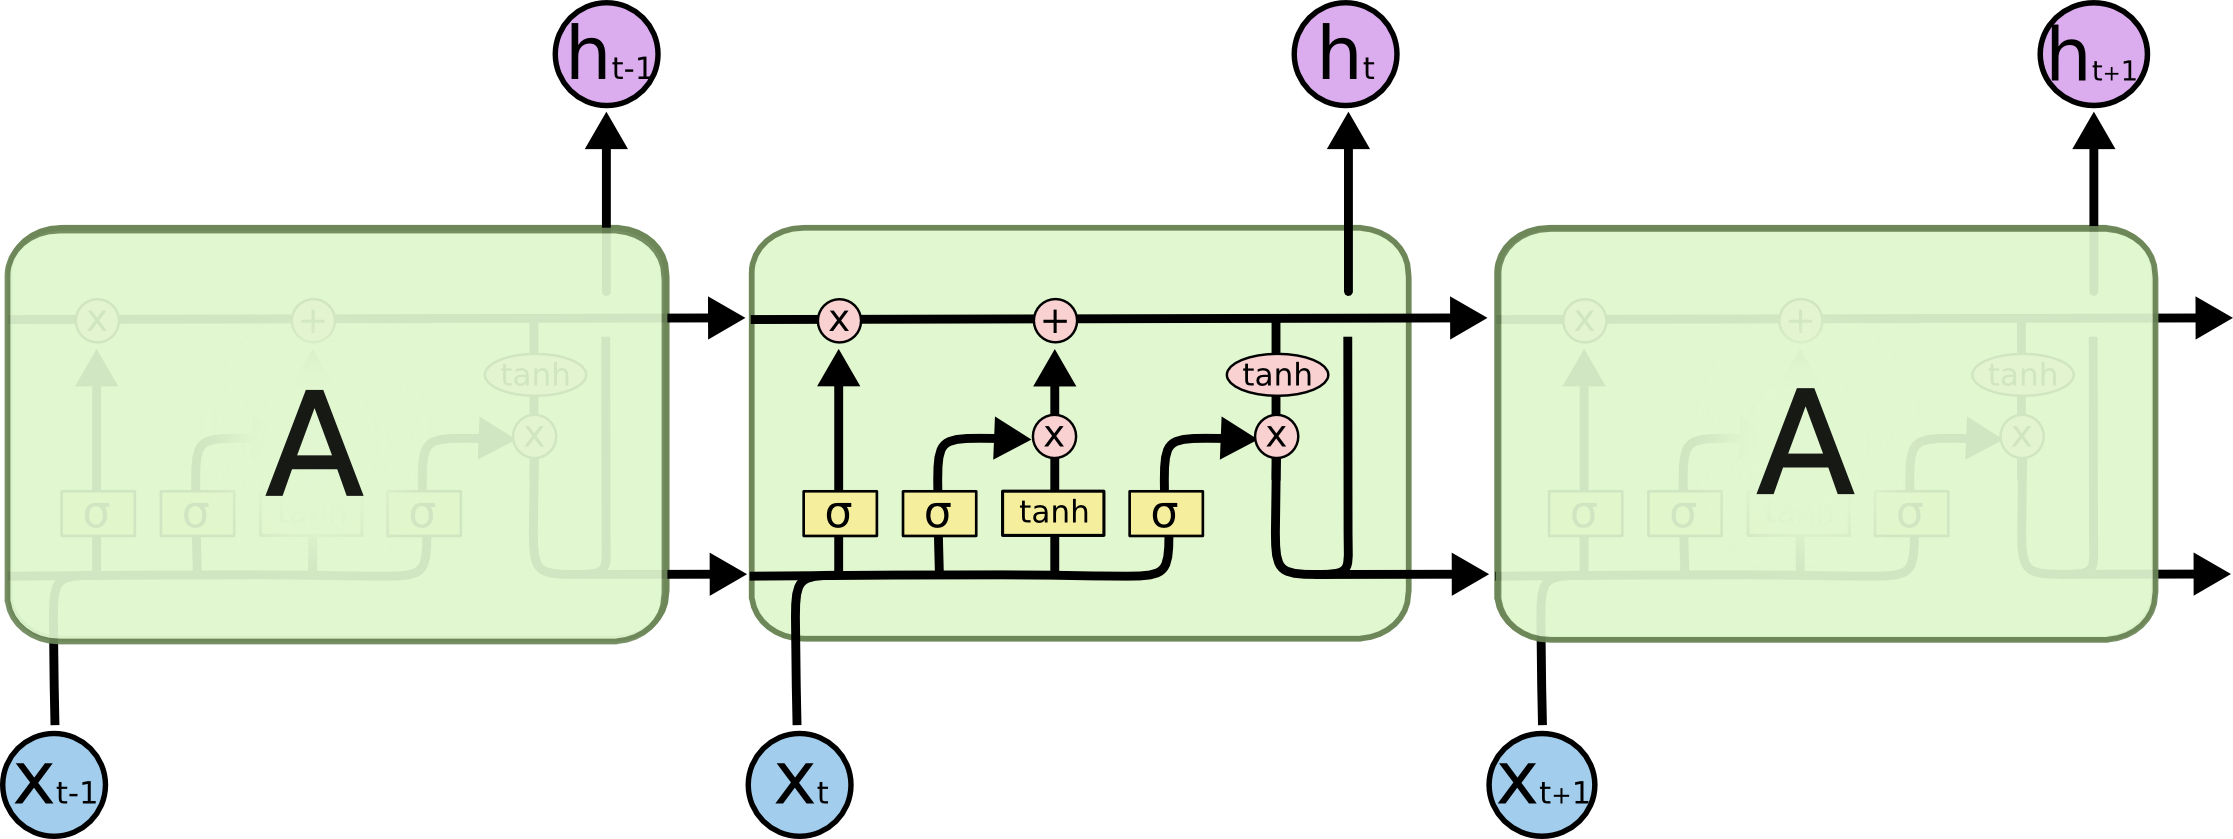
\includegraphics[width=0.8\textwidth]{LSTM-chain.png}
\caption{Internal structure of an LSTM unit, illustrating the flow of data and the gating mechanisms. Inputs  are processed alongside hidden states  and cell states , showcasing how information is selectively retained or discarded. Adapted from \cite{olah2015lstm}.}
\label{fig:lstm_structure}
\end{figure}

In this study, LSTMs are employed to forecast intraday stock price movements based on historical VWAP and trade count data. The model’s ability to capture complex, non-linear dependencies over a 3-hour look-back window makes it an ideal choice for this task. The architecture of the LSTM model is structured as follows:


\begin{itemize}
    \item \textbf{First LSTM Layer}: Contains 64 units and returns the full sequence of outputs, enabling further temporal processing.
    \item \textbf{Dropout Layer}: Applied with a 20\% dropout rate to the first LSTM layer’s output, reducing the risk of overfitting.
    \item \textbf{Second LSTM Layer}: Also with 64 units, this layer processes the sequence from the first layer and outputs only the final hidden state, summarizing the input sequence.
    \item \textbf{Second Dropout Layer}: Another 20\% dropout layer to further regularize the model.
    \item \textbf{Dense Output Layer}: A single-unit layer with a sigmoid activation function, producing the probability that the stock price will increase within the next three hours.
\end{itemize}

The model comprises 50,241 trainable parameters and is trained using BPTT with the Adam optimizer and binary cross-entropy loss function. To prevent overfitting and ensure efficient training, an EarlyStopping callback is employed to monitor validation accuracy, stopping the training process once improvements plateau and restoring the best weights. The input to the model is a matrix with 36 rows and 2 columns, where each row represents a 5-minute interval containing VWAP and trade count values, spanning a 3-hour look-back window (36 \(\times\) 5 minutes = 180 minutes).  The model’s output is a binary label— either 0 or 1 —indicating the predicted directional movement of the stock price in the next time interval, where 0 represents a decrease and 1 an increase. We adopt this binary classification approach because it reduces the complexity of the model and minimizes the impact of noise in financial data, allowing the model to focus on capturing underlying market trends and improving its predictive accuracy in a highly volatile and dynamic market. Moreover, this simplification is particularly advantageous in high-frequency trading environments, where predicting the direction of price change can be more actionable for traders than forecasting precise price values.

This LSTM architecture leverages its gating mechanisms to retain relevant patterns in the data while discarding noise, enabling accurate predictions of stock price movements. By processing sequences of intraday market data, the model captures the intricate temporal dynamics that drive financial markets, offering a powerful tool for forecasting.

\subsection{Evaluation Metrics}

To robustly and comprehensively evaluate predictive performance, we deployed a suite of carefully selected metrics:

\begin{itemize}[noitemsep]
  \item \textbf{Accuracy}: Assesses the overall proportion of correctly predicted directional outcomes, providing an aggregate measure of predictive efficacy.
  \item \textbf{Binary Cross‑Entropy Loss}: Evaluates the calibration, reliability, and confidence of probabilistic forecasts, ensuring accurate interpretation of predicted probabilities.
\end{itemize}

All model training and evaluation were performed on NVIDIA W100 GPUs to ensure efficient computation and reproducibility.

\section{Results}

Results are presented separately for the IEX and SIP datasets to investigate the influence of regular trading hours versus extended trading hours on model performance.

\subsection{IEX Data Evaluation}

For the IEX dataset, which includes only regular trading hours, the test accuracy and test loss are summarized in Tables~\ref{tab:iex_accuracy} and~\ref{tab:iex_loss}, respectively.


\begin{table}[H]
  \centering
  \definecolor{lightgreen}{RGB}{198, 255, 221}
      \caption{IEX Feed: Test Accuracy by Scaler and Ticker (Including Mean)}
  \begin{tabular}{lcccc}
  \toprule
  \textbf{Ticker} & \textbf{Standard} & \textbf{MinMax} & \textbf{Robust} & \textbf{NoScaler} \\
  \midrule
  AAPL  & 0.7370 & 0.7370 & \cellcolor{lightgreen}{0.7380} & 0.7230 \\
  AMZN  & 0.7330 & \cellcolor{lightgreen}{0.7500} & 0.7170 & 0.7170 \\
  DIA   & 0.5940 & \cellcolor{lightgreen}{0.6810} & 0.6680 & 0.6030 \\
  GOOG  & 0.5830 & 0.5880 & \cellcolor{lightgreen!30}0.5980 & 0.5710 \\
  IWM   & 0.6900 & 0.7110 & \cellcolor{lightgreen}{0.7160} & 0.6900 \\
  MSFT  & 0.7260 & 0.7350 & \cellcolor{lightgreen}{0.7370} & 0.7190 \\
  NVDA  & 0.7040 & \cellcolor{lightgreen}{0.7290} & 0.6220 & 0.6390 \\
  VOO   & 0.5930 & 0.5800 & 0.6050 & \cellcolor{lightgreen}{0.5850} \\
  \midrule
  \textbf{Mean} & 0.6700 & 0.6889 & 0.6751 & 0.6659 \\
  \bottomrule
  \label{tab:iex_accuracy}
  \end{tabular}
  \end{table}

\begin{table}[H]
\centering
\definecolor{lightblue}{RGB}{198, 221, 255}
\caption{IEX Feed: Test Loss by Scaler and Ticker (Including Mean)}
\begin{tabular}{lcccc}
\toprule
\textbf{Ticker} & \textbf{Standard} & \textbf{MinMax} & \textbf{Robust} & \textbf{NoScaler} \\
\midrule
AAPL  & 0.5510 & \cellcolor{lightblue}{0.5430} & 0.5530 & 0.5520 \\
AMZN  & \cellcolor{lightblue}0.5540 & 0.5560 & 0.5840 & 0.8200 \\
DIA   & 0.7270 & 0.6850 & 0.7080 & \cellcolor{lightblue}{0.6590} \\
GOOG  & 0.6560 & \cellcolor{lightblue}{0.5900} & 0.6320 & 0.6850 \\
IWM   & 0.6120 & 0.5980 & 0.6110 &\cellcolor{lightblue} 0.5870 \\
MSFT  & 0.6140 & \cellcolor{lightblue}{0.5360} & 0.5850 & 0.5410 \\
NVDA  & \cellcolor{lightblue}0.5450 & 0.5460 & 0.5490 & 0.6090 \\
VOO   & \cellcolor{lightblue}{0.6730} & 0.6940 & 0.6840 & 0.6800 \\
\midrule
\textbf{Mean} & 0.6165 & \cellcolor{lightblue}{0.5935} & 0.6133 & 0.6416 \\
\bottomrule
\label{tab:iex_loss}
\end{tabular}
\end{table}

\subsubsection*{Key Observations for IEX}

\textbf{Test Accuracy:} The MinMax scaler achieved the highest mean accuracy (0.6981), outperforming Standard (0.6838), Robust (0.6797), and NoScaler (0.6744). At the ticker-specific level, MinMax was optimal for AAPL, GOOG and NVDA, while the Robust scaler excelled for AMZN and MSFT. NoScaler provided the best accuracy for DIA and IWM, and the Standard scaler was the most effective only for VOO. This variation highlights the importance of selecting appropriate scaling methods based on individual stocks or ETFs.

\textbf{Test Loss:} MinMax also had the lowest mean loss (0.5935), clearly outperforming Standard (0.6165), Robust (0.6133), and NoScaler (0.6416). Ticker-specific analysis shows MinMax performed best for AAPL, GOOG and MSFT, while NoScaler was optimal for DIA and IWM. Standard scaling achieved the lowest loss values for AMZN, NVDA and VOO. These results confirm MinMax as generally effective in reducing loss during regular trading hours, despite some exceptions across tickers.

\subsection{SIP Data Evaluation}

For the SIP dataset, which includes extended trading hours (pre-market, regular and post-market sessions), the test accuracy and test loss are summarized in Tables~\ref{tab:sip_accuracy} and~\ref{tab:sip_loss}, respectively.

\begin{table}[H]
\centering
\caption{SIP Feed: Test Accuracy by Scaler and Ticker (Including Mean)}
\begin{tabular}{lcccc}
\toprule
\textbf{Ticker} & \textbf{Standard} & \textbf{MinMax} & \textbf{Robust} & \textbf{NoScaler} \\
\midrule 
AAPL & 0.8230 & 0.8310 & 0.8400 & \cellcolor{green!30} 0.8440 \\ 
AMZN & 0.7900 & 0.7930 & 0.7910 & \cellcolor{green!30} 0.8000 \\ 
DIA  & 0.8300 & 0.8370 & 0.8360 & \cellcolor{green!30} 0.8390 \\ 
GOOG & 0.8080 & \cellcolor{green!30}0.8160 & \cellcolor{green!30}0.8160 & 0.8070 \\ 
IWM  & 0.8120 & 0.8120 & 0.8050 & \cellcolor{green!30}0.8240 \\ 
MSFT & 0.8540 & 0.8520 & 0.8500 & \cellcolor{green!30} 0.8600 \\ 
NVDA & \cellcolor{green!30}0.8410 & 0.8340 & 0.8360 & 0.8400 \\ 
VOO  & 0.8730 & 0.8600 & \cellcolor{green!30}0.8740 & 0.8700 \\ 
\midrule
Mean & 0.8289 & 0.8294 & 0.8310 & \cellcolor{green!30} 0.8355 \\ 
\bottomrule
\label{tab:sip_accuracy}
\end{tabular}
\end{table}

\begin{table}[H]
  \centering
  \caption{SIP Feed: Test Loss by Scaler and Ticker (Including Mean)}
  \begin{tabular}{lcccc}
  \toprule
  \textbf{Ticker} & \textbf{Standard} & \textbf{MinMax} & \textbf{Robust} & \textbf{NoScaler} \\ 
  \midrule
  AAPL & 0.5580 & \cellcolor{blue!30} 0.4080 & 0.4230 & 0.4140 \\ 
  AMZN & 0.7180 & 0.6130 & 0.6490 & \cellcolor{blue!30} 0.6050 \\
  DIA  & 0.3880 & 0.3830 & 0.4040 & \cellcolor{blue!30} 0.3720 \\ 
  GOOG & \cellcolor{blue!30} 0.5590 & 0.6090 & 0.5770 & 0.6070 \\ 
  IWM  & 0.4690 & 0.4720 & 0.7410 & \cellcolor{blue!30}0.3890 \\ 
  MSFT & 0.3730 & 0.3680 & 0.3650 & \cellcolor{blue!30} 0.3460 \\ 
  NVDA & 0.3720 & 0.3770 & 0.3890 & \cellcolor{blue!30} 0.3670 \\ 
  VOO  & 0.3200 & 0.3170 & 0.3560 & \cellcolor{blue!30} 0.2940 \\ 
  \midrule
  Mean & 0.4696 & 0.4443 & 0.4880 & \cellcolor{blue!30} 0.4243 \\
  \bottomrule
  \label{tab:sip_loss}
  \end{tabular}
  \end{table}

\subsubsection*{Key Observations for SIP}

\textbf{Test Accuracy:} The Standard scaler produced the highest mean accuracy (0.8179), surpassing Robust (0.8164), MinMax (0.8156), and NoScaler (0.7871). For individual tickers, NoScaler provided the highest accuracy for AAPL, DIA, and IWM. Robust scaling performed best for AMZN, MSFT, and VOO, while Standard scaling excelled for GOOG and tied with MinMax for NVDA. These findings suggest that while the Standard scaler generally delivers the best performance, NoScaler remains competitive for certain tickers, particularly ETFs.

\textbf{Test Loss:} The Standard scaler recorded a mean loss of 0.4534, outperforming MinMax (0.4761), Robust (0.4657), and NoScaler (0.5301). For individual tickers, NoScaler produced the lowest loss for AAPL, DIA and IWM while Robust scaling achieved the lowest loss for AMZN, GOOG and MSFT. The Standard scaler performed best for NVDA, VOO and tied with Robust in AMZN. These results suggest that while Standard scaling delivers the lowest loss for several tickers, NoScaler is particularly effective for certain ETFs, particularly DIA and IWM, where it outperforms other scalers.

%Tabela e graficos do SP500.

%Colocar imagem do sp500 durante 2016 ate 2024

\section{Discussion}

\subsection{Performance Across Data Feeds} 

A central outcome of this investigation is the clear performance advantage achieved by incorporating extended trading sessions through the use of SIP data. Models trained on SIP data consistently outperformed their counterparts trained on IEX data across both mean test accuracy and loss. The top-performing configuration—Robust scaling applied to SIP—achieved a mean accuracy of 0.8201, outperforming the best IEX configuration (MinMax scaling, 0.6981 mean accuracy) by a substantial margin. This suggests that off-hours trading—despite its increased complexity—contains valuable predictive signals for short-horizon price forecasting.

The SIP dataset captures market dynamics that are often absent during standard trading hours, including early institutional positioning, overnight macroeconomic shock assimilation, and post-close retail activity. These phenomena introduce temporal heterogeneity into the data, increasing both the richness and variance of the observed sequences. As a result, models trained on SIP data benefit from exposure to a broader set of market states, enhancing their ability to learn nuanced representations of regime transitions and anomalous behavior.

Nevertheless, this expanded temporal context also amplifies modeling challenges. Extended sessions exhibit elevated volatility, sparser liquidity, and more frequent structural breaks, which may violate implicit assumptions of local stationarity and smooth feature evolution. These conditions demand more robust preprocessing strategies. In our analysis, the Robust scaler proved particularly effective under these conditions, consistently outperforming alternative scalers in both accuracy and loss metrics. This affirms the utility of robust normalization in mitigating distributional shifts and handling heavy-tailed data typical of extended-hour market environments.

Figures~\ref{fig:scaler_comparison} and~\ref{fig:accuracy_improvement} visually summarize these results. The former compares mean accuracy across both datasets for each scaler, while the latter presents per‐ticker percentage improvement in predictive performance when transitioning from IEX to SIP. Most assets benefited meaningfully from SIP‐based training, affirming the generality of these findings.

A notable exception is NVDA, which exhibited a decline in model accuracy (-5.30\%) when trained on SIP data. This deviation likely reflects NVDA’s elevated exposure to high‐impact, unscheduled information events—such as earnings calls and product launches—which often occur during extended hours and introduce discontinuities in price dynamics. These regime changes disrupt temporal coherence and degrade the effectiveness of autoregressive models that assume locally smooth transitions. This case reinforces the importance of tailoring data inclusion strategies to asset‐specific characteristics such as news sensitivity and volatility clustering.

\begin{figure}[H]
    \centering
    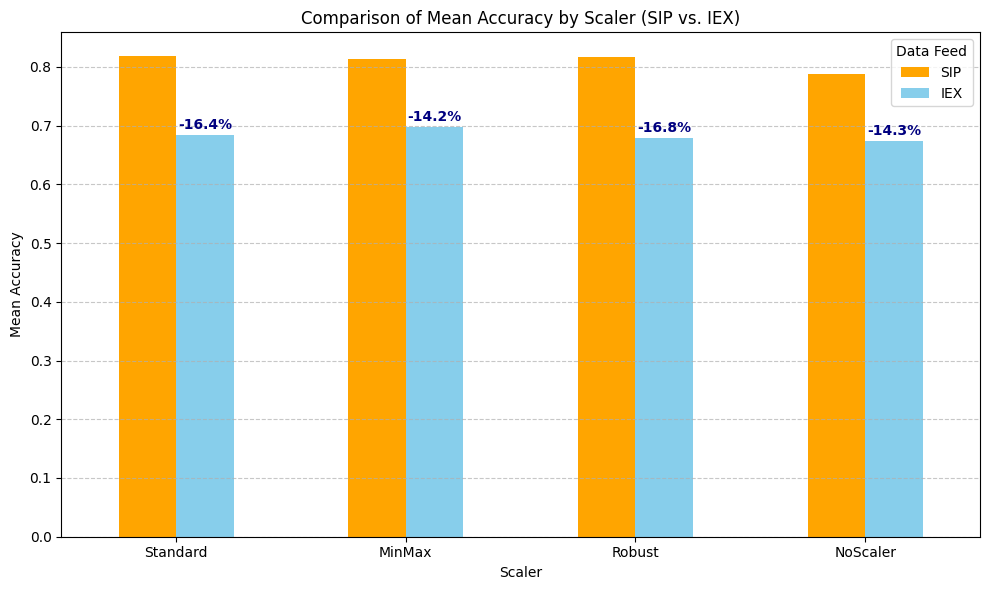
\includegraphics[width=0.95\textwidth]{scaler_comparison.png}
    \caption{Comparison of mean accuracy and loss by scaler between IEX and SIP datasets.}
    \label{fig:scaler_comparison}
\end{figure}

\begin{figure}[H]
    \centering
    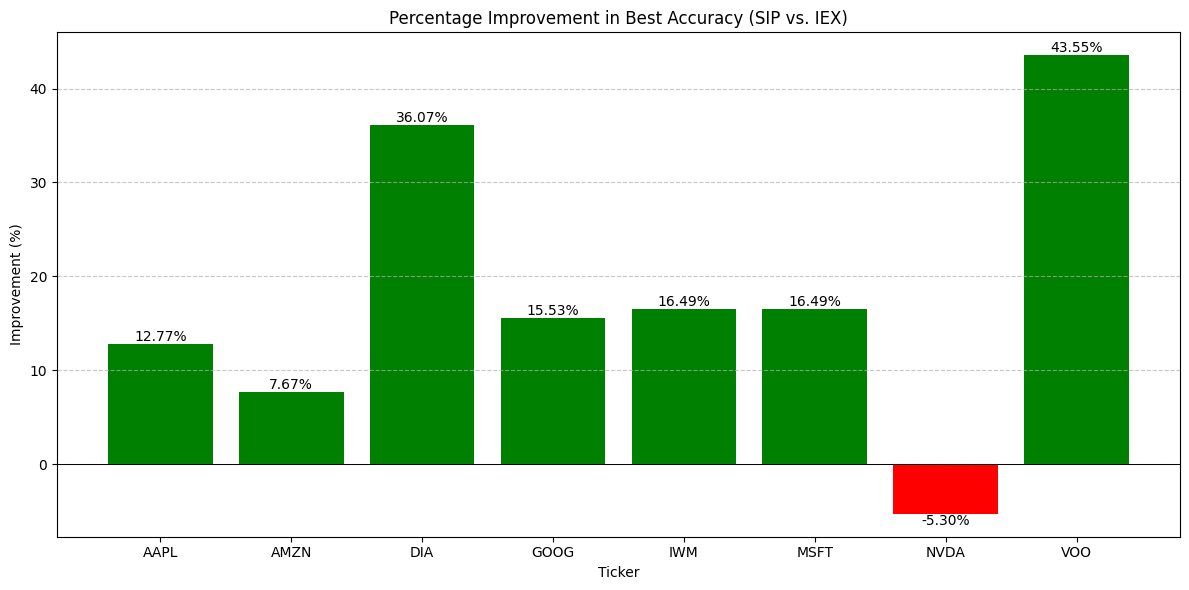
\includegraphics[width=1\textwidth]{accuracy_improvement.png}
    \caption{Percentage improvement in best accuracy per ticker from IEX to SIP. Positive values indicate improved accuracy with SIP data.}
    \label{fig:accuracy_improvement}
\end{figure}

Taken together, these findings suggest that while extended-session data generally enhances predic
tive accuracy, its benefits are not uniform across assets. The value of this information is contingent
 upon an asset’s volatility profile, liquidity regime, and sensitivity to exogenous events. As such, fu
ture implementations would benefit from adaptive, asset-aware data conditioning that dynamically
 determines which temporal segments to emphasize.

\subsection{Effectiveness of Scaling Techniques}

Across both the IEX and SIP datasets, data normalization significantly influenced model accuracy and stability, with the optimal scaling technique varying by dataset and asset type. For the IEX dataset, which covers only regular trading hours, the MinMax scaler proved most effective, achieving a mean test accuracy of 0.6981 and a mean test loss of 0.5935. This scaler normalizes features to a fixed range, making it well-suited to the relatively stable and bounded price movements typical of regular trading hours. By reducing the impact of minor fluctuations, the MinMax scaler enhances the model’s ability to detect consistent patterns in this less volatile environment.

In contrast, for the SIP dataset, although the Standard scaler produced the highest mean accuracy (0.8179) and the lowest mean loss (0.4534), the Robust scaler emerged as the best choice for mitigating volatility during extended hours, yielding a mean test accuracy of 0.8164 and a mean test loss of 0.4454. Extended hours often feature lower liquidity, leading to increased volatility, outliers, and price spikes. The Robust scaler, which relies on the median and interquartile range, mitigates the influence of these anomalies, providing a more stable foundation for model predictions. This explains its advantage over alternatives like the MinMax scaler (0.8156 accuracy, 0.4547 loss) and Standard scaler (0.8143 accuracy, 0.4571 loss) in certain tickers of the SIP dataset.

An additional insight from this analysis is the strong performance of the NoScaler configuration for specific asset classes, particularly ETFs. In both datasets, NoScaler achieved top-tier performance for instruments such as DIA, IWM, and VOO, reaching 0.8420, 0.8430, and 0.8750 accuracy in the SIP dataset. These instruments, by design, aggregate the performance of multiple underlying stocks, producing smoother price trajectories with reduced idiosyncratic volatility. The structural stability of ETFs appears to reduce the necessity for normalization, as the raw feature values already conform to a relatively low-noise distribution.

In these low-volatility regimes, normalization may in fact attenuate informative signals, particularly those embedded in the raw scale or directionality of inputs. By preserving the native feature structure, NoScaler can retain subtle dynamics that inform directional shifts, especially in assets with mean-reverting behavior. This suggests that the application of normalization should be conditioned on asset-specific properties, including volatility clustering, mean-reversion strength, and exposure to external news shocks.

These findings collectively argue for a flexible and adaptive approach to preprocessing in financial deep learning. While MinMax and Robust scalers are highly effective in regular and extended sessions respectively, their blanket application may obscure latent structure in instruments with inherently stable dynamics. An ideal system would employ context-aware preprocessing, selecting or blending scalers based on real-time diagnostics of data distribution properties.

\subsection{Volatility}

To rigorously investigate the role of asset-specific volatility in shaping the predictive performance
of LSTM models, we computed annualized volatility estimates for each ticker over the test window
spanning June 7, 2023, to December 30, 2024. In quantitative finance, volatility is convention
ally defined as the standard deviation of returns and serves as a widely accepted proxy for risk.
Elevated volatility is associated with amplified uncertainty, reflecting greater dispersion in return
sequences driven by exogenous market events. From a forecasting perspective, such volatility com
plicates pattern recognition, introduces structural nonstationarity, and degrades the learnability
of temporal dependencies—posing significant challenges for recurrent models like LSTMs.

Annualized volatility was calculated using a three-step procedure grounded in standard financial
 econometrics, specifically leveraging log return statistics:

\begin{enumerate}
    \item \textbf{Compute daily log returns:}
    \begin{equation}
    R_t = \ln\left(\frac{P_t}{P_{t-1}}\right),
    \end{equation}
    where \(P_t\) and \(P_{t-1}\) represent closing prices on days \(t\) and \(t-1\), respectively.


    
    \item \textbf{Calculate daily volatility (\(\sigma_{\text{daily}}\)):}
    \begin{equation}
    \sigma_{\text{daily}} = \sqrt{\frac{1}{n-1}\sum_{t=1}^{n}(R_t - \bar{R})^2},
    \end{equation}
    with \(\bar{R}\) as the average daily log return.

    \item \textbf{Annualize daily volatility assuming 252 trading days per year:}
    \begin{equation}
    \sigma_{\text{annualized}} = \sigma_{\text{daily}} \times \sqrt{252}.
    \end{equation}
\end{enumerate}

We then analyzed the correlation between annualized volatility and the best test accuracy, defined as the highest accuracy achieved by the LSTM model for each ticker during the testing phase. As shown in Figure~\ref{fig:volatility_accuracy}, a negative correlation emerged. Highly volatile stocks, such as NVDA, exhibited lower predictive accuracy compared to less volatile tickers like VOO, DIA and MSFT. This suggests that elevated volatility increases the unpredictability of price movements, challenging the LSTM model's ability to identify reliable patterns.

\begin{figure}[H]
    \centering
    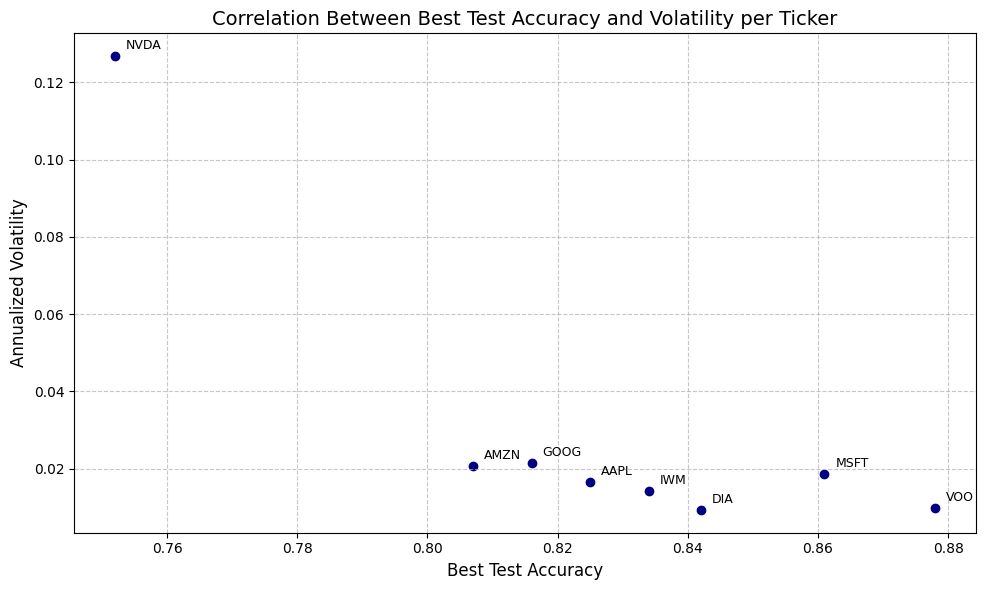
\includegraphics[width=1\textwidth]{volatility_accuracy.png}
    \caption{Correlation between annualized volatility and best test accuracy across tickers. Higher volatility typically corresponds to reduced predictive accuracy.}
    \label{fig:volatility_accuracy}
\end{figure}

The case of NVDA is particularly illustrative. This asset exhibited the highest annualized volatility within the sample and correspondingly the lowest LSTM-based accuracy. NVDA’s volatility profile is likely attributable to recurrent firm-specific events, such as earnings announcements, product innovations, and macro-sensitive sectoral dynamics—many of which occur during extended trading sessions. These events introduce abrupt discontinuities and fat-tailed return behavior that violate the temporal smoothness assumptions inherent in recurrent models. Furthermore, NVDA’s performance degraded under the SIP data regime, suggesting that extended-hour volatility amplifies noise and reduces forecastability for highly reactive equities.

Conversely, ETFs such as VOO and DIA demonstrated both low volatility and high predictive accuracy. These instruments track broad market indices, inherently reducing exposure to idiosyncratic events and yielding smoother return distributions. This dampening of firm-specific risk translates into more stationary temporal sequences, facilitating the LSTM’s ability to extract and retain predictive structure. The contrast between NVDA and diversified ETFs thus reinforces the conclusion that return volatility acts as a modulating factor in model learnability.

We further analyzed how volatility interacts with feature scaling. Preliminary evidence indicates that scaling strategies exhibit volatility sensitivity: the Robust scaler consistently improved model stability in high-volatility environments due to its resistance to outliers and skew, while the NoScaler approach outperformed alternatives in low-volatility contexts by preserving raw price magnitudes that may encode directionally relevant signals. These findings suggest that preprocessing pipelines should be volatility-aware, dynamically adapting scaler selection based on asset-level return distribution diagnostics.

In aggregate, these results underscore that volatility is not a passive attribute but an active determinant of neural model performance. Highly volatile assets introduce representational challenges that necessitate architectural and algorithmic adaptations. Potential solutions include incorporating volatility as an auxiliary input feature, utilizing regime-switching models that adjust learning dynamics based on return variance, or employing attention mechanisms that prioritize temporally stable subsequences. Additionally, custom loss functions that penalize misclassification in volatile regimes more heavily could steer training dynamics toward robustness.

As financial markets become increasingly nonlinear and event-driven, forecasting in high-volatility environments will demand models that are not only statistically expressive but also contextually responsive. Building architectures that condition on asset-specific volatility—whether via exogenous features, adaptive training protocols, or hybrid preprocessing strategies—will be crucial for advancing the frontier of deep learning in quantitative finance.

\section{Future Improvements}

While this study demonstrates the potential of LSTM networks in predicting short-term stock price movements, there are several avenues for future improvements and extensions that could further enhance the accuracy and robustness of the model.

\subsection{Incorporating More Advanced Feature Engineering}
One potential improvement is the inclusion of additional features derived from both financial and non-financial data sources. While this study uses VWAP and trade count as key microstructure features, adding other technical indicators such as the Relative Strength Index (RSI), Moving Averages, Bollinger Bands, and MACD could provide a more complete view of market dynamics. Furthermore, sentiment analysis derived from financial news, earnings reports, or social media could provide critical insights into market psychology and drive further improvements in predictive accuracy. Incorporating external macroeconomic variables such as GDP growth, inflation rates, and interest rates could also help the model better account for broader market movements.

\subsection{Expanding the Model to Hybrid Architectures}
Although LSTM networks have shown strong performance, there may be room for improvement by exploring hybrid models. Combining LSTM with other neural architectures, such as Convolutional Neural Networks (CNN) for spatial feature extraction or attention mechanisms for focusing on the most important features, could enhance the model’s ability to capture both temporal and spatial dependencies in financial data. For instance, a CNN-LSTM hybrid could first extract key patterns from the raw data and then pass them to the LSTM to capture long-term dependencies.

\subsection{Model Evaluation and Backtesting}
Another area for improvement is the comprehensive evaluation of the model’s real-world applicability. While the study has conducted extensive testing on historical data, future work should incorporate rigorous backtesting within a simulated trading environment. This would enable an assessment of how well the model performs when used to inform trading decisions, factoring in transaction costs, slippage, and other market frictions. Further real-time testing with paper trading or live trading could provide valuable insights into the model’s performance under actual market conditions, especially during periods of high volatility.

\subsection{Improving Model Interpretability}
One challenge with deep learning models, including LSTMs, is their inherent lack of interpretability. Understanding the reasons behind a model’s prediction is critical in financial applications, where decisions can have significant financial consequences. Future work could explore techniques for improving the interpretability of the model. One promising direction is to integrate attention mechanisms into the LSTM architecture to highlight which parts of the input data (e.g., specific time intervals or features like VWAP) are most influential in the model’s decision-making process. Additionally, using methods such as SHAP (SHapley Additive exPlanations) or LIME (Local Interpretable Model-Agnostic Explanations) could help explain the model's outputs in a more transparent and actionable way.

\section{Conclusion}

This study presented a comprehensive and methodologically rigorous evaluation of LSTM networks for the task of intraday stock price prediction, emphasizing the influence of data normalization techniques, trading session structure, and asset-specific volatility profiles. By systematically analyzing model behavior across datasets representing both regular trading hours (IEX) and full-session trading (SIP), the investigation provides nuanced insights into the design and deployment of deep learning models in high-frequency financial forecasting.

Empirical results consistently demonstrated that the inclusion of extended trading sessions significantly improved predictive performance. LSTM models trained on SIP data achieved higher accuracy than their IEX-based counterparts across nearly all assets, affirming that pre-market and post-market activity, despite its elevated noise and reduced liquidity, contributes valuable information to the price discovery process. These findings support the assertion that enhanced temporal resolution and broader market coverage increase the richness of training signals available to deep learning models.

The study further identified a pronounced interaction between normalization strategy and trading regime. MinMax scaling performed best in the context of regular trading hours, where price dynamics are comparatively smooth and bounded. Conversely, Robust scaling excelled in the SIP dataset, where volatility, outlier frequency, and distributional skew are elevated. This performance dichotomy underscores the importance of context-aware preprocessing pipelines that adapt to both market structure and the statistical properties of the input data.

Additionally, certain asset classes—particularly ETFs such as DIA, VOO, and IWM—achieved optimal results without any feature scaling. These instruments, by virtue of their diversified exposure and reduced idiosyncratic noise, generate smoother return sequences that appear to benefit from retaining the raw scale of input features. This suggests that preprocessing decisions should be conditioned not only on volatility regime but also on instrument type, as normalization may suppress valuable signal structure in certain contexts.

Volatility emerged as a central determinant of model generalization. A strong inverse correlation was observed between annualized volatility and best test accuracy, with highly volatile stocks such as NVDA displaying notably lower predictive performance. These assets are more susceptible to event-driven shocks and structural breaks, which compromise the temporal coherence upon which LSTM models rely. Such findings highlight the limitations of static model architectures and motivate the development of volatility-aware mechanisms capable of dynamically adjusting to shifts in return distributions.

%Several promising avenues for future research emerge from this work. Meta-learning approaches could facilitate joint optimization of model weights and preprocessing parameters, automating the selection of scalers based on data-driven criteria. Additionally, incorporating auxiliary inputs—such as realized or implied volatility estimates, sentiment indices, or macroeconomic event indicators—may further enhance model adaptability. Attention-based architectures and regime-switching frameworks could also be leveraged to improve temporal sensitivity and robustness in the presence of structural market changes.

In summary, this study underscores that high-performing financial forecasting with LSTM models requires a holistic approach—one that integrates flexible architectural design with adaptive preprocessing and asset-specific contextualization. As financial markets grow increasingly complex, fragmented, and sensitive to exogenous stimuli, the capacity to construct forecasting systems that intelligently align with the evolving structure of the data will be essential. Advancements in this area will depend on the synergistic integration of algorithmic expressiveness, domain-specific feature engineering, and real-time adaptivity, enabling the construction of robust, interpretable, and scalable predictive frameworks for dynamic financial environments.

\newpage

\section{Attachments}

\subsection{Parameter Exploration}\label{subsec:parameter_exploration}

The pipeline constitutes a fully automated, end-to-end framework that ingests market data, applies user-defined preprocessing and feature-engineering steps, constructs sequential tensors, configures and trains an LSTM network (or alternative model), and produces all evaluation artifacts and reports—entirely driven by a single \texttt{config} dictionary.  By exposing every critical choice (data source, symbols, date range, feature markers, scaling strategy, model hyperparameters, etc.) as configurable parameters, users can rapidly iterate on their hypotheses without modifying any core code.

\begin{itemize}[left=0pt]
       \item \texttt{data\_source} (\texttt{'sip'}, \texttt{'iex'}): choice of data provider.
       \item \texttt{symbol} (e.g.\ \texttt{'AAPL'}): ticker symbol to fetch, or read from an Excel file.
       \item \texttt{max\_period} (\texttt{True}, \texttt{False}): whether to request the entire available history (be mindful of API rate limits).
       \item \texttt{start\_date}, \texttt{end\_date} (e.g.\ \texttt{'2022-10-31'}–\texttt{'2023-10-31'}): date range for the backtest; one year is a good default for experimentation.
       \item \texttt{timeframe} (\texttt{'1Min'}, \texttt{'5Min'}): sampling interval for bars.
       \item \texttt{first\_marker}, \texttt{second\_marker}, \texttt{third\_marker} (e.g.\ \texttt{'trade\_count'}, \texttt{'vwap'}, \texttt{'volume'}): columns used as “channels” in the tensor; start with trade count and VWAP, and optionally add a third if it empirically improves performance.
       \item \texttt{n\_rows} (e.g.\ 5, 12, 36): number of time‑steps in each tensor slice; 36 performed best in our tests, but you should align this with your chosen timeframe.
       \item \texttt{sort} (\texttt{True}, \texttt{False}): whether to sort the dataset by its second column before constructing tensors.
       \item \texttt{adjustment} (\texttt{all}, \texttt{split}, \texttt{dividend}, \texttt{none}): type of adjustment to apply to the data.
       \item \texttt{relative\_first\_marker}, \texttt{relative\_second\_marker}, \texttt{relative\_third\_marker} (\texttt{True}, \texttt{False}): apply relative normalization per marker across the tensor—you’ll need empirical evidence to decide which channels benefit from relative scaling.
       \item \texttt{decimals} (e.g.\ \texttt{3}, \texttt{4}): number of decimal places to round to; small rounding can sometimes stabilize training.
       \item \texttt{scaler\_type} (\texttt{'none'}, \texttt{'minmax'}, \texttt{'standard'}, \texttt{'maxabs'}, \texttt{'robust'}, \texttt{'quantile'}, \texttt{'power'}, \texttt{'normalize'}, \texttt{'binarizer'}): choice of feature scaler for your dataset.
       \item \texttt{cols\_to\_scale} (\texttt{None}, \texttt{[0]}, \texttt{[0,1]}, …): which columns to apply the scaler to—\texttt{None} means all.
       \item \texttt{LSTM\_boolean} (\texttt{True}, \texttt{False}): whether to build and train an LSTM; disabling it can test non-sequential baselines.
       \item \texttt{epochs} (e.g.\ 5, 50, 500): maximum training epochs; early checkpoints mean this is often just an upper bound.
       \item \texttt{early\_stopping} (\texttt{True}, \texttt{False}): toggle automatic early stopping.
       \item \texttt{call\_back} (\texttt{'val\_accuracy'}, \texttt{'val\_loss'}, \texttt{'accuracy'}, \texttt{'loss'}): metric to monitor for early stopping.
       \item \texttt{patience} (e.g.\ 2, 100, 1000): number of epochs without improvement before halting.
       \item \texttt{batch\_size} (e.g.\ 16, 64, 512): size of training batches; larger batches can speed up training on large datasets.
   
\end{itemize}

This flexibility allows to tailor data sourcing, feature construction, normalization, and training dynamics to experimental needs.

For the models used in this paper, the following settings were applied:

\begin{itemize} [left=0pt]
  \item \texttt{max\_period}: \texttt{False} – Only a specified date range was used for backtesting. 
  \item \texttt{start\_date}: \texttt{'2016-01-01'} – Data fetching started from January 1, 2016. 
  \item \texttt{end\_date}: \texttt{'2024-12-30'} – The backtest period concluded on December 30, 2024. 
  \item \texttt{timeframe}: \texttt{'5Min'} – A 5-minute sampling interval was used to capture intraday price movements. 
  \item \texttt{first\_marker}: \texttt{'vwap'} – Volume-Weighted Average Price was used as the first feature. 
  \item \texttt{second\_marker}: \texttt{'trade\_count'} – Trade count was used as the second feature. 
  \item \texttt{third\_marker}: Not used in the experiments. 
  \item \texttt{n\_rows}: \texttt{36} – The model was configured to use 36 time-steps in each tensor slice. 
  \item \texttt{sort}: \texttt{False} – No sorting of data was applied before constructing tensors. 
  \item \texttt{adjustment}: \texttt{'all'} – All types of adjustments (such as split and dividend) were applied to the data. 
  \item \texttt{relative\_first\_marker}: \texttt{False} – No relative normalization was applied to the first marker (VWAP). 
  \item \texttt{relative\_second\_marker}: \texttt{False} – No relative normalization was applied to the second marker (trade count). 
  \item \texttt{relative\_third\_marker}: \texttt{False} – No relative normalization was applied to the third marker. 
  \item \texttt{decimals}: \texttt{4} – Data was rounded to 4 decimal places to stabilize training.  
  \item \texttt{cols\_to\_scale}: \texttt{[0]} – Scaling was applied only to the first column (VWAP). 
  \item \texttt{LSTM\_boolean}: \texttt{True} – Long Short-Term Memory networks were employed for the predictions. 
  \item \texttt{epochs}: \texttt{500} – A maximum of 500 epochs was set for model training. 
  \item \texttt{early\_stopping}: \texttt{True} – Early stopping was enabled to halt training once validation accuracy stopped improving. 
  \item \texttt{call\_back}: \texttt{'val\_accuracy'} – Validation accuracy was monitored for early stopping. 
  \item \texttt{patience}: \texttt{100} – The model was allowed to train for 100 epochs without improvement before early stopping was triggered. 
  \item \texttt{batch\_size}: \texttt{128} – A batch size of 128 was used during training for efficient learning. 
\end{itemize}

\textbf{Note:} The \texttt{data\_source} and \texttt{symbol} parameters were varied throughout the experiments, with both data sources (SIP and IEX) and different ticker symbols (e.g., AAPL, AMZN, and VOO) tested in various runs to evaluate model robustness across datasets. Similarly, the \texttt{scaler\_type} parameter was tested with different scaling strategies, including Standard, MinMax, and Robust scaling, to analyze their impact on the model's performance.


\subsection{Algorithm}\label{subsec:lstm_pipeline}

Below is a high-level algorithmic representation of the LSTM model training and saving pipeline, along with the corresponding diagram. The algorithm outlines the key steps involved in the process, from data fetching to model evaluation and saving, while the diagram visually represents the workflow, providing a clearer understanding of the sequence of actions.

\begin{algorithm}[H]
\caption{LSTM Model Training and Saving Pipeline}
\label{alg:lstm_pipeline}
\begin{algorithmic}[1]
    \State \textbf{Step 1: Set Up Directory Paths}
    \State \hspace{1em} Initialize path variables

    \State \textbf{Step 2: Set Up Configuration}
    \State \hspace{1em} Initialize configuration variables:
    \Statex \hspace{2em}\texttt{data\_source}, \texttt{symbol}, \texttt{max\_period}, \texttt{start\_date}, \texttt{end\_date}, \texttt{timeframe}
    \Statex \hspace{2em}\texttt{fisrt\_marker}, \texttt{second\_marker}, \texttt{third\_marker}
    \Statex \hspace{2em}\texttt{n\_rows}, \texttt{sort}, \texttt{adjustment}
    \Statex \hspace{2em}\texttt{relative\_first\_marker}, \texttt{relative\_second\_marker}, \texttt{relative\_third\_marker}
    \Statex \hspace{2em}\texttt{decimals}
    \Statex \hspace{2em}\texttt{scaler\_type}, \texttt{cols\_to\_scale}
    \Statex \hspace{2em}\texttt{LSTM\_boolean}, \texttt{epochs}, \texttt{early\_stopping}, \texttt{call\_back}, \texttt{patience}, \texttt{batch\_size}

    \State \textbf{Step 3: Load or Fetch Data}
    \If{\texttt{dataset.csv} exists}
        \State Read raw data from CSV at \texttt{dataset.csv}
    \Else
        \State Fetch data from Alpaca API using \texttt{data\_source}, \texttt{symbol}, \texttt{start\_date}, \texttt{end\_date}, \texttt{timeframe}, \texttt{max\_period}
        \State Save raw data to \texttt{dataset.csv}
    \EndIf

    \State \textbf{Step 4: Scale Selected Features}
    \State \hspace{1em} Initialize scaler of type \texttt{scaler\_type} on columns \texttt{cols\_to\_scale}
    \State \hspace{1em} Fit and transform the data (respecting \texttt{relative\_*} flags and \texttt{decimals})
    \State \hspace{1em} Save fitted scaler

    \State \textbf{Step 5: Build and Compile LSTM Model}
    \State \hspace{1em} Define LSTM architecture if \texttt{LSTM\_boolean} is \texttt{True}
    \State \hspace{1em} Compile model with chosen loss and optimizer

    \State \textbf{Step 6: Train Model}
    \State \hspace{1em} Train for \texttt{epochs} epochs with:
    \Statex \hspace{2em}\texttt{batch\_size}, early stopping on \texttt{call\_back} with \texttt{patience}
    \State \hspace{1em} Record training history (loss, accuracy)

    \State \textbf{Step 7: Generate Evaluation Artifacts}
    \State \hspace{1em} Plot loss and accuracy curves
    \State \hspace{1em} Compute confusion matrix
    \State \hspace{1em} Save all plots

    \State \textbf{Step 8: Save Outputs}
    \State \hspace{1em} Save trained model
    \State \hspace{1em} Save \texttt{config}
    \State \hspace{1em} Generate and save HTML report (including paths, \texttt{config}, plots, confusion matrix)

\end{algorithmic}
\end{algorithm}


\begin{figure}[H]
  \centering
  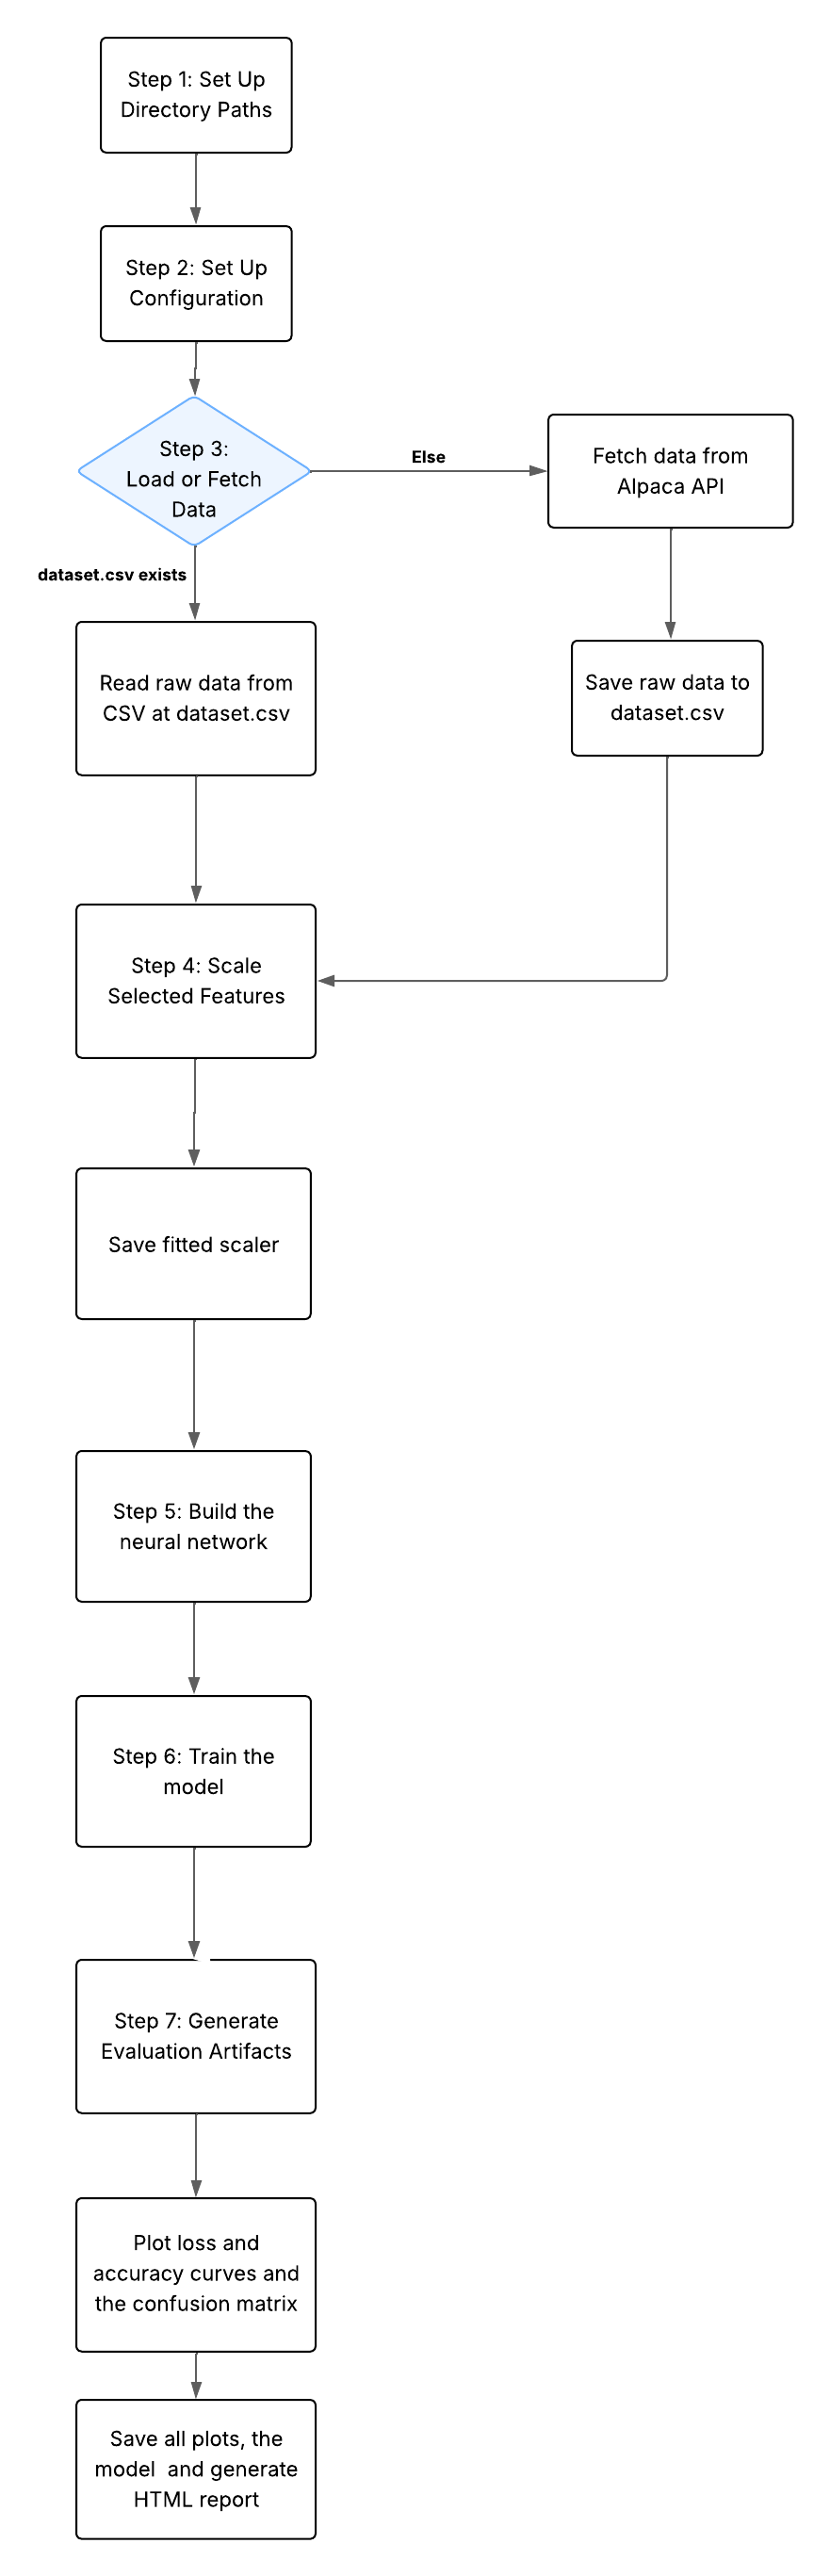
\includegraphics[width=0.48\textwidth]{diagram.png}
  \caption{Diagram of the LSTM pipeline.}
  \label{fig:lstm_pipeline}
\end{figure}

\subsection{Tickers}

The following figures illustrate the performance of the LSTM model across different tickers and scaling methods. Each figure includes three subplots: accuracy, loss, and confusion matrix (CM).
\subsubsection{AAPL}
\begin{figure}[H]
  \centering
  \includegraphics[width=0.32\linewidth]{IEX/Robust/AAPL/aapl_iex_robust_accuracy.png}
  \includegraphics[width=0.32\linewidth]{IEX/Robust/AAPL/aapl_iex_robust_loss.png}
  \includegraphics[width=0.32\linewidth]{IEX/Robust/AAPL/aapl_iex_robust_cm.png}
  \caption{AAPL – IEX – Robust Scaling}
\end{figure}
\begin{figure}[H]
  \centering
  \includegraphics[width=0.32\linewidth]{IEX/NoScaler/AAPL/aapl_iex_noscaler_accuracy.png}
  \includegraphics[width=0.32\linewidth]{IEX/NoScaler/AAPL/aapl_iex_noscaler_loss.png}
  \includegraphics[width=0.32\linewidth]{IEX/NoScaler/AAPL/aapl_iex_noscaler_cm.png}
  \caption{AAPL – IEX – NoScaler}
\end{figure}
\begin{figure}[H]
  \centering
  \includegraphics[width=0.32\linewidth]{IEX/MinMax/AAPL/aapl_iex_minmax_accuracy.png}
  \includegraphics[width=0.32\linewidth]{IEX/MinMax/AAPL/aapl_iex_minmax_loss.png}
  \includegraphics[width=0.32\linewidth]{IEX/MinMax/AAPL/aapl_iex_minmax_cm.png}
  \caption{AAPL – IEX – MinMax Scaling}
\end{figure}
\begin{figure}[H]
  \centering
  \includegraphics[width=0.32\linewidth]{IEX/Standard/AAPL/aapl_iex_standard_accuracy.png}
  \includegraphics[width=0.32\linewidth]{IEX/Standard/AAPL/aapl_iex_standard_loss.png}
  \includegraphics[width=0.32\linewidth]{IEX/Standard/AAPL/aapl_iex_standard_cm.png}
  \caption{AAPL – IEX – Standard Scaling}
\end{figure}
\begin{figure}[H]
  \centering
  \includegraphics[width=0.32\linewidth]{SIP/Robust/AAPL/aapl_sip_robust_accuracy.png}
  \includegraphics[width=0.32\linewidth]{SIP/Robust/AAPL/aapl_sip_robust_loss.png}
  \includegraphics[width=0.32\linewidth]{SIP/Robust/AAPL/aapl_sip_robust_cm.png}
  \caption{AAPL – SIP – Robust Scaling}
\end{figure}
\begin{figure}[H]
  \centering
  \includegraphics[width=0.32\linewidth]{SIP/NoScaler/AAPL/aapl_sip_noscaler_accuracy.png}
  \includegraphics[width=0.32\linewidth]{SIP/NoScaler/AAPL/aapl_sip_noscaler_loss.png}
  \includegraphics[width=0.32\linewidth]{SIP/NoScaler/AAPL/aapl_sip_noscaler_cm.png}
  \caption{AAPL – SIP – NoScaler}
\end{figure}
\begin{figure}[H]
  \centering
  \includegraphics[width=0.32\linewidth]{SIP/MinMax/AAPL/aapl_sip_minmax_accuracy.png}
  \includegraphics[width=0.32\linewidth]{SIP/MinMax/AAPL/aapl_sip_minmax_loss.png}
  \includegraphics[width=0.32\linewidth]{SIP/MinMax/AAPL/aapl_sip_minmax_cm.png}
  \caption{AAPL – SIP – MinMax Scaling}
\end{figure}
\begin{figure}[H]
  \centering
  \includegraphics[width=0.32\linewidth]{SIP/Standard/AAPL/aapl_sip_standard_accuracy.png}
  \includegraphics[width=0.32\linewidth]{SIP/Standard/AAPL/aapl_sip_standard_loss.png}
  \includegraphics[width=0.32\linewidth]{SIP/Standard/AAPL/aapl_sip_standard_cm.png}
  \caption{AAPL – SIP – Standard Scaling}
\end{figure}

\subsubsection{AMZN}
\begin{figure}[H]
  \centering
  \includegraphics[width=0.32\linewidth]{IEX/Robust/AMZN/amzn_iex_robust_accuracy.png}
  \includegraphics[width=0.32\linewidth]{IEX/Robust/AMZN/amzn_iex_robust_loss.png}
  \includegraphics[width=0.32\linewidth]{IEX/Robust/AMZN/amzn_iex_robust_cm.png}
  \caption{AMZN – IEX – Robust Scaling}
\end{figure}
\begin{figure}[H]
  \centering
  \includegraphics[width=0.32\linewidth]{IEX/NoScaler/AMZN/amzn_iex_noscaler_accuracy.png}
  \includegraphics[width=0.32\linewidth]{IEX/NoScaler/AMZN/amzn_iex_noscaler_loss.png}
  \includegraphics[width=0.32\linewidth]{IEX/NoScaler/AMZN/amzn_iex_noscaler_cm.png}
  \caption{AMZN – IEX – NoScaler}
\end{figure}
\begin{figure}[H]
  \centering
  \includegraphics[width=0.32\linewidth]{IEX/MinMax/AMZN/amzn_iex_minmax_accuracy.png}
  \includegraphics[width=0.32\linewidth]{IEX/MinMax/AMZN/amzn_iex_minmax_loss.png}
  \includegraphics[width=0.32\linewidth]{IEX/MinMax/AMZN/amzn_iex_minmax_cm.png}
  \caption{AMZN – IEX – MinMax Scaling}
\end{figure}
\begin{figure}[H]
  \centering
  \includegraphics[width=0.32\linewidth]{IEX/Standard/AMZN/amzn_iex_standard_accuracy.png}
  \includegraphics[width=0.32\linewidth]{IEX/Standard/AMZN/amzn_iex_standard_loss.png}
  \includegraphics[width=0.32\linewidth]{IEX/Standard/AMZN/amzn_iex_standard_cm.png}
  \caption{AMZN – IEX – Standard Scaling}
\end{figure}
\begin{figure}[H]
  \centering
  \includegraphics[width=0.32\linewidth]{SIP/Robust/AMZN/amzn_sip_robust_accuracy.png}
  \includegraphics[width=0.32\linewidth]{SIP/Robust/AMZN/amzn_sip_robust_loss.png}
  \includegraphics[width=0.32\linewidth]{SIP/Robust/AMZN/amzn_sip_robust_cm.png}
  \caption{AMZN – SIP – Robust Scaling}
\end{figure}
\begin{figure}[H]
  \centering
  \includegraphics[width=0.32\linewidth]{SIP/NoScaler/AMZN/amzn_sip_noscaler_accuracy.png}
  \includegraphics[width=0.32\linewidth]{SIP/NoScaler/AMZN/amzn_sip_noscaler_loss.png}
  \includegraphics[width=0.32\linewidth]{SIP/NoScaler/AMZN/amzn_sip_noscaler_cm.png}
  \caption{AMZN – SIP – NoScaler}
\end{figure}
\begin{figure}[H]
  \centering
  \includegraphics[width=0.32\linewidth]{SIP/MinMax/AMZN/amzn_sip_minmax_accuracy.png}
  \includegraphics[width=0.32\linewidth]{SIP/MinMax/AMZN/amzn_sip_minmax_loss.png}
  \includegraphics[width=0.32\linewidth]{SIP/MinMax/AMZN/amzn_sip_minmax_cm.png}
  \caption{AMZN – SIP – MinMax Scaling}
\end{figure}
\begin{figure}[H]
  \centering
  \includegraphics[width=0.32\linewidth]{SIP/Standard/AMZN/amzn_sip_standard_accuracy.png}
  \includegraphics[width=0.32\linewidth]{SIP/Standard/AMZN/amzn_sip_standard_loss.png}
  \includegraphics[width=0.32\linewidth]{SIP/Standard/AMZN/amzn_sip_standard_cm.png}
  \caption{AMZN – SIP – Standard Scaling}
\end{figure}

\subsubsection{DIA}
\begin{figure}[H]
  \centering
  \includegraphics[width=0.32\linewidth]{IEX/Robust/DIA/dia_iex_robust_accuracy.png}
  \includegraphics[width=0.32\linewidth]{IEX/Robust/DIA/dia_iex_robust_loss.png}
  \includegraphics[width=0.32\linewidth]{IEX/Robust/DIA/dia_iex_robust_cm.png}
  \caption{DIA – IEX – Robust Scaling}
\end{figure}
\begin{figure}[H]
  \centering
  \includegraphics[width=0.32\linewidth]{IEX/NoScaler/DIA/dia_iex_noscaler_accuracy.png}
  \includegraphics[width=0.32\linewidth]{IEX/NoScaler/DIA/dia_iex_noscaler_loss.png}
  \includegraphics[width=0.32\linewidth]{IEX/NoScaler/DIA/dia_iex_noscaler_cm.png}
  \caption{DIA – IEX – NoScaler}
\end{figure}
\begin{figure}[H]
  \centering
  \includegraphics[width=0.32\linewidth]{IEX/MinMax/DIA/dia_iex_minmax_accuracy.png}
  \includegraphics[width=0.32\linewidth]{IEX/MinMax/DIA/dia_iex_minmax_loss.png}
  \includegraphics[width=0.32\linewidth]{IEX/MinMax/DIA/dia_iex_minmax_cm.png}
  \caption{DIA – IEX – MinMax Scaling}
\end{figure}
\begin{figure}[H]
  \centering
  \includegraphics[width=0.32\linewidth]{IEX/Standard/DIA/dia_iex_standard_accuracy.png}
  \includegraphics[width=0.32\linewidth]{IEX/Standard/DIA/dia_iex_standard_loss.png}
  \includegraphics[width=0.32\linewidth]{IEX/Standard/DIA/dia_iex_standard_cm.png}
  \caption{DIA – IEX – Standard Scaling}
\end{figure}
\begin{figure}[H]
  \centering
  \includegraphics[width=0.32\linewidth]{SIP/Robust/DIA/dia_sip_robust_accuracy.png}
  \includegraphics[width=0.32\linewidth]{SIP/Robust/DIA/dia_sip_robust_loss.png}
  \includegraphics[width=0.32\linewidth]{SIP/Robust/DIA/dia_sip_robust_cm.png}
  \caption{DIA – SIP – Robust Scaling}
\end{figure}
\begin{figure}[H]
  \centering
  \includegraphics[width=0.32\linewidth]{SIP/NoScaler/DIA/dia_sip_noscaler_accuracy.png}
  \includegraphics[width=0.32\linewidth]{SIP/NoScaler/DIA/dia_sip_noscaler_loss.png}
  \includegraphics[width=0.32\linewidth]{SIP/NoScaler/DIA/dia_sip_noscaler_cm.png}
  \caption{DIA – SIP – NoScaler}
\end{figure}
\begin{figure}[H]
  \centering
  \includegraphics[width=0.32\linewidth]{SIP/MinMax/DIA/dia_sip_minmax_accuracy.png}
  \includegraphics[width=0.32\linewidth]{SIP/MinMax/DIA/dia_sip_minmax_loss.png}
  \includegraphics[width=0.32\linewidth]{SIP/MinMax/DIA/dia_sip_minmax_cm.png}
  \caption{DIA – SIP – MinMax Scaling}
\end{figure}
\begin{figure}[H]
  \centering
  \includegraphics[width=0.32\linewidth]{SIP/Standard/DIA/dia_sip_standard_accuracy.png}
  \includegraphics[width=0.32\linewidth]{SIP/Standard/DIA/dia_sip_standard_loss.png}
  \includegraphics[width=0.32\linewidth]{SIP/Standard/DIA/dia_sip_standard_cm.png}
  \caption{DIA – SIP – Standard Scaling}
\end{figure}

\subsubsection{GOOG}
\begin{figure}[H]
  \centering
  \includegraphics[width=0.32\linewidth]{IEX/Robust/GOOG/goog_iex_robust_accuracy.png}
  \includegraphics[width=0.32\linewidth]{IEX/Robust/GOOG/goog_iex_robust_loss.png}
  \includegraphics[width=0.32\linewidth]{IEX/Robust/GOOG/goog_iex_robust_cm.png}
  \caption{GOOG – IEX – Robust Scaling}
\end{figure}
\begin{figure}[H]
  \centering
  \includegraphics[width=0.32\linewidth]{IEX/NoScaler/GOOG/goog_iex_noscaler_accuracy.png}
  \includegraphics[width=0.32\linewidth]{IEX/NoScaler/GOOG/goog_iex_noscaler_loss.png}
  \includegraphics[width=0.32\linewidth]{IEX/NoScaler/GOOG/goog_iex_noscaler_cm.png}
  \caption{GOOG – IEX – NoScaler}
\end{figure}
\begin{figure}[H]
  \centering
  \includegraphics[width=0.32\linewidth]{IEX/MinMax/GOOG/goog_iex_minmax_accuracy.png}
  \includegraphics[width=0.32\linewidth]{IEX/MinMax/GOOG/goog_iex_minmax_loss.png}
  \includegraphics[width=0.32\linewidth]{IEX/MinMax/GOOG/goog_iex_minmax_cm.png}
  \caption{GOOG – IEX – MinMax Scaling}
\end{figure}
\begin{figure}[H]
  \centering
  \includegraphics[width=0.32\linewidth]{IEX/Standard/GOOG/goog_iex_standard_accuracy.png}
  \includegraphics[width=0.32\linewidth]{IEX/Standard/GOOG/goog_iex_standard_loss.png}
  \includegraphics[width=0.32\linewidth]{IEX/Standard/GOOG/goog_iex_standard_cm.png}
  \caption{GOOG – IEX – Standard Scaling}
\end{figure}
\begin{figure}[H]
  \centering
  \includegraphics[width=0.32\linewidth]{SIP/Robust/GOOG/goog_sip_robust_accuracy.png}
  \includegraphics[width=0.32\linewidth]{SIP/Robust/GOOG/goog_sip_robust_loss.png}
  \includegraphics[width=0.32\linewidth]{SIP/Robust/GOOG/goog_sip_robust_cm.png}
  \caption{GOOG – SIP – Robust Scaling}
\end{figure}
\begin{figure}[H]
  \centering
  \includegraphics[width=0.32\linewidth]{SIP/NoScaler/GOOG/goog_sip_noscaler_accuracy.png}
  \includegraphics[width=0.32\linewidth]{SIP/NoScaler/GOOG/goog_sip_noscaler_loss.png}
  \includegraphics[width=0.32\linewidth]{SIP/NoScaler/GOOG/goog_sip_noscaler_cm.png}
  \caption{GOOG – SIP – NoScaler}
\end{figure}
\begin{figure}[H]
  \centering
  \includegraphics[width=0.32\linewidth]{SIP/MinMax/GOOG/goog_sip_minmax_accuracy.png}
  \includegraphics[width=0.32\linewidth]{SIP/MinMax/GOOG/goog_sip_minmax_loss.png}
  \includegraphics[width=0.32\linewidth]{SIP/MinMax/GOOG/goog_sip_minmax_cm.png}
  \caption{GOOG – SIP – MinMax Scaling}
\end{figure}
\begin{figure}[H]
  \centering
  \includegraphics[width=0.32\linewidth]{SIP/Standard/GOOG/goog_sip_standard_accuracy.png}
  \includegraphics[width=0.32\linewidth]{SIP/Standard/GOOG/goog_sip_standard_loss.png}
  \includegraphics[width=0.32\linewidth]{SIP/Standard/GOOG/goog_sip_standard_cm.png}
  \caption{GOOG – SIP – Standard Scaling}
\end{figure}

\subsubsection{IWM}
\begin{figure}[H]
  \centering
  \includegraphics[width=0.32\linewidth]{IEX/Robust/IWM/iwm_iex_robust_accuracy.png}
  \includegraphics[width=0.32\linewidth]{IEX/Robust/IWM/iwm_iex_robust_loss.png}
  \includegraphics[width=0.32\linewidth]{IEX/Robust/IWM/iwm_iex_robust_cm.png}
  \caption{IWM – IEX – Robust Scaling}
\end{figure}
\begin{figure}[H]
  \centering
  \includegraphics[width=0.32\linewidth]{IEX/NoScaler/IWM/iwm_iex_noscaler_accuracy.png}
  \includegraphics[width=0.32\linewidth]{IEX/NoScaler/IWM/iwm_iex_noscaler_loss.png}
  \includegraphics[width=0.32\linewidth]{IEX/NoScaler/IWM/iwm_iex_noscaler_cm.png}
  \caption{IWM – IEX – NoScaler}
\end{figure}
\begin{figure}[H]
  \centering
  \includegraphics[width=0.32\linewidth]{IEX/MinMax/IWM/iwm_iex_minmax_accuracy.png}
  \includegraphics[width=0.32\linewidth]{IEX/MinMax/IWM/iwm_iex_minmax_loss.png}
  \includegraphics[width=0.32\linewidth]{IEX/MinMax/IWM/iwm_iex_minmax_cm.png}
  \caption{IWM – IEX – MinMax Scaling}
\end{figure}
\begin{figure}[H]
  \centering
  \includegraphics[width=0.32\linewidth]{IEX/Standard/IWM/iwm_iex_standard_accuracy.png}
  \includegraphics[width=0.32\linewidth]{IEX/Standard/IWM/iwm_iex_standard_loss.png}
  \includegraphics[width=0.32\linewidth]{IEX/Standard/IWM/iwm_iex_standard_cm.png}
  \caption{IWM – IEX – Standard Scaling}
\end{figure}
\begin{figure}[H]
  \centering
  \includegraphics[width=0.32\linewidth]{SIP/Robust/IWM/iwm_sip_robust_accuracy.png}
  \includegraphics[width=0.32\linewidth]{SIP/Robust/IWM/iwm_sip_robust_loss.png}
  \includegraphics[width=0.32\linewidth]{SIP/Robust/IWM/iwm_sip_robust_cm.png}
  \caption{IWM – SIP – Robust Scaling}
\end{figure}
\begin{figure}[H]
  \centering
  \includegraphics[width=0.32\linewidth]{SIP/NoScaler/IWM/iwm_sip_noscaler_accuracy.png}
  \includegraphics[width=0.32\linewidth]{SIP/NoScaler/IWM/iwm_sip_noscaler_loss.png}
  \includegraphics[width=0.32\linewidth]{SIP/NoScaler/IWM/iwm_sip_noscaler_cm.png}
  \caption{IWM – SIP – NoScaler}
\end{figure}
\begin{figure}[H]
  \centering
  \includegraphics[width=0.32\linewidth]{SIP/MinMax/IWM/iwm_sip_minmax_accuracy.png}
  \includegraphics[width=0.32\linewidth]{SIP/MinMax/IWM/iwm_sip_minmax_loss.png}
  \includegraphics[width=0.32\linewidth]{SIP/MinMax/IWM/iwm_sip_minmax_cm.png}
  \caption{IWM – SIP – MinMax Scaling}
\end{figure}
\begin{figure}[H]
  \centering
  \includegraphics[width=0.32\linewidth]{SIP/Standard/IWM/iwm_sip_standard_accuracy.png}
  \includegraphics[width=0.32\linewidth]{SIP/Standard/IWM/iwm_sip_standard_loss.png}
  \includegraphics[width=0.32\linewidth]{SIP/Standard/IWM/iwm_sip_standard_cm.png}
  \caption{IWM – SIP – Standard Scaling}
\end{figure}

\subsubsection{MSFT}
\begin{figure}[H]
  \centering
  \includegraphics[width=0.32\linewidth]{IEX/Robust/MSFT/msft_iex_robust_accuracy.png}
  \includegraphics[width=0.32\linewidth]{IEX/Robust/MSFT/msft_iex_robust_loss.png}
  \includegraphics[width=0.32\linewidth]{IEX/Robust/MSFT/msft_iex_robust_cm.png}
  \caption{MSFT – IEX – Robust Scaling}
\end{figure}
\begin{figure}[H]
  \centering
  \includegraphics[width=0.32\linewidth]{IEX/NoScaler/MSFT/msft_iex_noscaler_accuracy.png}
  \includegraphics[width=0.32\linewidth]{IEX/NoScaler/MSFT/msft_iex_noscaler_loss.png}
  \includegraphics[width=0.32\linewidth]{IEX/NoScaler/MSFT/msft_iex_noscaler_cm.png}
  \caption{MSFT – IEX – NoScaler}
\end{figure}
\begin{figure}[H]
  \centering
  \includegraphics[width=0.32\linewidth]{IEX/MinMax/MSFT/msft_iex_minmax_accuracy.png}
  \includegraphics[width=0.32\linewidth]{IEX/MinMax/MSFT/msft_iex_minmax_loss.png}
  \includegraphics[width=0.32\linewidth]{IEX/MinMax/MSFT/msft_iex_minmax_cm.png}
  \caption{MSFT – IEX – MinMax Scaling}
\end{figure}
\begin{figure}[H]
  \centering
  \includegraphics[width=0.32\linewidth]{IEX/Standard/MSFT/msft_iex_standard_accuracy.png}
  \includegraphics[width=0.32\linewidth]{IEX/Standard/MSFT/msft_iex_standard_loss.png}
  \includegraphics[width=0.32\linewidth]{IEX/Standard/MSFT/msft_iex_standard_cm.png}
  \caption{MSFT – IEX – Standard Scaling}
\end{figure}
\begin{figure}[H]
  \centering
  \includegraphics[width=0.32\linewidth]{SIP/Robust/MSFT/msft_sip_robust_accuracy.png}
  \includegraphics[width=0.32\linewidth]{SIP/Robust/MSFT/msft_sip_robust_loss.png}
  \includegraphics[width=0.32\linewidth]{SIP/Robust/MSFT/msft_sip_robust_cm.png}
  \caption{MSFT – SIP – Robust Scaling}
\end{figure}
\begin{figure}[H]
  \centering
  \includegraphics[width=0.32\linewidth]{SIP/NoScaler/MSFT/msft_sip_noscaler_accuracy.png}
  \includegraphics[width=0.32\linewidth]{SIP/NoScaler/MSFT/msft_sip_noscaler_loss.png}
  \includegraphics[width=0.32\linewidth]{SIP/NoScaler/MSFT/msft_sip_noscaler_cm.png}
  \caption{MSFT – SIP – NoScaler}
\end{figure}
\begin{figure}[H]
  \centering
  \includegraphics[width=0.32\linewidth]{SIP/MinMax/MSFT/msft_sip_minmax_accuracy.png}
  \includegraphics[width=0.32\linewidth]{SIP/MinMax/MSFT/msft_sip_minmax_loss.png}
  \includegraphics[width=0.32\linewidth]{SIP/MinMax/MSFT/msft_sip_minmax_cm.png}
  \caption{MSFT – SIP – MinMax Scaling}
\end{figure}
\begin{figure}[H]
  \centering
  \includegraphics[width=0.32\linewidth]{SIP/Standard/MSFT/msft_sip_standard_accuracy.png}
  \includegraphics[width=0.32\linewidth]{SIP/Standard/MSFT/msft_sip_standard_loss.png}
  \includegraphics[width=0.32\linewidth]{SIP/Standard/MSFT/msft_sip_standard_cm.png}
  \caption{MSFT – SIP – Standard Scaling}
\end{figure}

\subsubsection{NVDA}
\begin{figure}[H]
  \centering
  \includegraphics[width=0.32\linewidth]{IEX/Robust/NVDA/nvda_iex_robust_accuracy.png}
  \includegraphics[width=0.32\linewidth]{IEX/Robust/NVDA/nvda_iex_robust_loss.png}
  \includegraphics[width=0.32\linewidth]{IEX/Robust/NVDA/nvda_iex_robust_cm.png}
  \caption{NVDA – IEX – Robust Scaling}
\end{figure}
\begin{figure}[H]
  \centering
  \includegraphics[width=0.32\linewidth]{IEX/NoScaler/NVDA/nvda_iex_noscaler_accuracy.png}
  \includegraphics[width=0.32\linewidth]{IEX/NoScaler/NVDA/nvda_iex_noscaler_loss.png}
  \includegraphics[width=0.32\linewidth]{IEX/NoScaler/NVDA/nvda_iex_noscaler_cm.png}
  \caption{NVDA – IEX – NoScaler}
\end{figure}
\begin{figure}[H]
  \centering
  \includegraphics[width=0.32\linewidth]{IEX/MinMax/NVDA/nvda_iex_minmax_accuracy.png}
  \includegraphics[width=0.32\linewidth]{IEX/MinMax/NVDA/nvda_iex_minmax_loss.png}
  \includegraphics[width=0.32\linewidth]{IEX/MinMax/NVDA/nvda_iex_minmax_cm.png}
  \caption{NVDA – IEX – MinMax Scaling}
\end{figure}
\begin{figure}[H]
  \centering
  \includegraphics[width=0.32\linewidth]{IEX/Standard/NVDA/nvda_iex_standard_accuracy.png}
  \includegraphics[width=0.32\linewidth]{IEX/Standard/NVDA/nvda_iex_standard_loss.png}
  \includegraphics[width=0.32\linewidth]{IEX/Standard/NVDA/nvda_iex_standard_cm.png}
  \caption{NVDA – IEX – Standard Scaling}
\end{figure}
\begin{figure}[H]
  \centering
  \includegraphics[width=0.32\linewidth]{SIP/Robust/NVDA/nvda_sip_robust_accuracy.png}
  \includegraphics[width=0.32\linewidth]{SIP/Robust/NVDA/nvda_sip_robust_loss.png}
  \includegraphics[width=0.32\linewidth]{SIP/Robust/NVDA/nvda_sip_robust_cm.png}
  \caption{NVDA – SIP – Robust Scaling}
\end{figure}
\begin{figure}[H]
  \centering
  \includegraphics[width=0.32\linewidth]{SIP/NoScaler/NVDA/nvda_sip_noscaler_accuracy.png}
  \includegraphics[width=0.32\linewidth]{SIP/NoScaler/NVDA/nvda_sip_noscaler_loss.png}
  \includegraphics[width=0.32\linewidth]{SIP/NoScaler/NVDA/nvda_sip_noscaler_cm.png}
  \caption{NVDA – SIP – NoScaler}
\end{figure}
\begin{figure}[H]
  \centering
  \includegraphics[width=0.32\linewidth]{SIP/MinMax/NVDA/nvda_sip_minmax_accuracy.png}
  \includegraphics[width=0.32\linewidth]{SIP/MinMax/NVDA/nvda_sip_minmax_loss.png}
  \includegraphics[width=0.32\linewidth]{SIP/MinMax/NVDA/nvda_sip_minmax_cm.png}
  \caption{NVDA – SIP – MinMax Scaling}
\end{figure}
\begin{figure}[H]
  \centering
  \includegraphics[width=0.32\linewidth]{SIP/Standard/NVDA/nvda_sip_standard_accuracy.png}
  \includegraphics[width=0.32\linewidth]{SIP/Standard/NVDA/nvda_sip_standard_loss.png}
  \includegraphics[width=0.32\linewidth]{SIP/Standard/NVDA/nvda_sip_standard_cm.png}
  \caption{NVDA – SIP – Standard Scaling}
\end{figure}

\subsubsection{VOO}
\begin{figure}[H]
  \centering
  \includegraphics[width=0.32\linewidth]{IEX/Robust/VOO/voo_iex_robust_accuracy.png}
  \includegraphics[width=0.32\linewidth]{IEX/Robust/VOO/voo_iex_robust_loss.png}
  \includegraphics[width=0.32\linewidth]{IEX/Robust/VOO/voo_iex_robust_cm.png}
  \caption{VOO – IEX – Robust Scaling}
\end{figure}
\begin{figure}[H]
  \centering
  \includegraphics[width=0.32\linewidth]{IEX/NoScaler/VOO/voo_iex_noscaler_accuracy.png}
  \includegraphics[width=0.32\linewidth]{IEX/NoScaler/VOO/voo_iex_noscaler_loss.png}
  \includegraphics[width=0.32\linewidth]{IEX/NoScaler/VOO/voo_iex_noscaler_cm.png}
  \caption{VOO – IEX – NoScaler}
\end{figure}
\begin{figure}[H]
  \centering
  \includegraphics[width=0.32\linewidth]{IEX/MinMax/VOO/voo_iex_minmax_accuracy.png}
  \includegraphics[width=0.32\linewidth]{IEX/MinMax/VOO/voo_iex_minmax_loss.png}
  \includegraphics[width=0.32\linewidth]{IEX/MinMax/VOO/voo_iex_minmax_cm.png}
  \caption{VOO – IEX – MinMax Scaling}
\end{figure}
\begin{figure}[H]
  \centering
  \includegraphics[width=0.32\linewidth]{IEX/Standard/VOO/voo_iex_standard_accuracy.png}
  \includegraphics[width=0.32\linewidth]{IEX/Standard/VOO/voo_iex_standard_loss.png}
  \includegraphics[width=0.32\linewidth]{IEX/Standard/VOO/voo_iex_standard_cm.png}
  \caption{VOO – IEX – Standard Scaling}
\end{figure}
\begin{figure}[H]
  \centering
  \includegraphics[width=0.32\linewidth]{SIP/Robust/VOO/voo_sip_robust_accuracy.png}
  \includegraphics[width=0.32\linewidth]{SIP/Robust/VOO/voo_sip_robust_loss.png}
  \includegraphics[width=0.32\linewidth]{SIP/Robust/VOO/voo_sip_robust_cm.png}
  \caption{VOO – SIP – Robust Scaling}
\end{figure}
\begin{figure}[H]
  \centering
  \includegraphics[width=0.32\linewidth]{SIP/NoScaler/VOO/voo_sip_noscaler_accuracy.png}
  \includegraphics[width=0.32\linewidth]{SIP/NoScaler/VOO/voo_sip_noscaler_loss.png}
  \includegraphics[width=0.32\linewidth]{SIP/NoScaler/VOO/voo_sip_noscaler_cm.png}
  \caption{VOO – SIP – NoScaler}
\end{figure}
\begin{figure}[H]
  \centering
  \includegraphics[width=0.32\linewidth]{SIP/MinMax/VOO/voo_sip_minmax_accuracy.png}
  \includegraphics[width=0.32\linewidth]{SIP/MinMax/VOO/voo_sip_minmax_loss.png}
  \includegraphics[width=0.32\linewidth]{SIP/MinMax/VOO/voo_sip_minmax_cm.png}
  \caption{VOO – SIP – MinMax Scaling}
\end{figure}
\begin{figure}[H]
  \centering
  \includegraphics[width=0.32\linewidth]{SIP/Standard/VOO/voo_sip_standard_accuracy.png}
  \includegraphics[width=0.32\linewidth]{SIP/Standard/VOO/voo_sip_standard_loss.png}
  \includegraphics[width=0.32\linewidth]{SIP/Standard/VOO/voo_sip_standard_cm.png}
  \caption{VOO – SIP – Standard Scaling}
\end{figure}

\newpage

\section*{Abbreviations}
\begin{description}[noitemsep,style=multiline,leftmargin=3cm,labelwidth=2.5cm]
    \item[LSTM] Long short‑term memory
    \item[RNN] Recurrent neural networks
    \item[SIP] Securities Information Processor
    \item[IEX] Investors Exchange
    \item[ETF] Exchange-traded fund
    \item[VWAP] Volume Weighted Average Price
    \item[VOO] Vanguard S\&P 500 ETF
    \item[DIA] SPDR Dow Jones Industrial Average ETF
    \item[IWM] iShares Russell 2000 ETF
    \item[AMZN] Amazon
    \item[AAPL] Apple
    \item[MSFT] Microsoft
    \item[GOOG] Alphabet
    \item[NVDA] Nvidia
    \item[EMH] Efficient Market Hypothesis
    \item[BPTT] Backpropagation Through Time
    \item[RSI] Relative Strength Index
    \item[MACD] Moving Average Convergence Divergence
    \item[SHAP] SHapley Additive exPlanations
    \item[LIME] Local Interpretable Model-Agnostic Explanations
    \item[CNN] Convolutional Neural Networks
    
\end{description}

\section*{Acknowledgements}
The authors would like to express their sincere gratitude to Imperial College London and Instituto Superior Técnico for their support and resources which were invaluable to this research.

Additionally, we acknowledge the use of Alpaca Trading API, TensorFlow and scikit-learn which were essential for conducting this study.

Finally, the authors wish to express their gratitude to their family, friends, and colleagues for the consistent encouragement and understanding provided throughout this research endeavour.

\section*{Authors’ contributions}
All authors have reviewed and approved the final version of the manuscript.

\section*{Competing interests}
The authors declare no competing interests.
%
% ---- Bibliography ----
%
% BibTeX users should specify bibliography style 'splncs04'.
% References will then be sorted and formatted in the correct style.

\bibliographystyle{splncs04}
\bibliography{referencias}

\end{document}
